\documentclass[DM,toc]{lsstdoc}

\setDocChangeRecord{%
\addtohist{1.1}{2004-06-23}{Initial version (Document-139).}{J.~Kantor}
\addtohist{1.2}{2011-07-12}{Updated for PDR.}{J.~Kantor}
\addtohist{1.3}{2014-03-07}{Updated for construction phase.}{J.~Kantor}
\addtohist{1.4}{2014-10-21}{SQuaRE section added.}{J.~Kantor}
\addtohist{1.5}{2014-10-30}{Added LDM-294 handle.}{J.~Kantor}
\addtohist{2.0}{2015-03-11}{Updated with new RFC process, realignment of TCT, SAT, DMLT.}{J.~Kantor}
\addtohist{3.0}{2017-06-30}{Complete overhaul of content, with all new authors. Rewritten in LaTeX. Approved for release by W.~O'Mullane.}{W.~O'Mullane}
\addtohist{3.1}{2017-07-04}{Minor cleanups for review. Approved in \jira{RFC-358}.}{W.~O'Mullane}
\addtohist{3.2}{2017-07-19}{Editorial fixes and refresh schedule and component  diagrams}{W.~O'Mullane}
\addtohist{3.3}{2017-08-21}{Update CCB and SE groups. Add Science Platform Scientist. Add section on design reviews. Approved in \jira{RFC-373}.}{W.~O'Mullane}
\addtohist{3.4}{2017-12-21}{Org chart refresh - rules for review of epics \jira{DM-7501}}{W.~O'Mullane}
\addtohist{3.5}{2018-06-18}{New DM product tree and revised org chart. Add deputy subsystem scientist. Approved in \jira{RFC-493}}{J.~Swinbank}
\addtohist{3.6}{2019-01-29}{Review product tree. Add release management subsection. Update DMCCB and DMSE team. Approved in \jira{RFC-561}}{G.~Comoretto}
\addtohist{3.7}{2019-02-06}{Add text for LSP and Middleware mangers. Time allocation policy for institutional scientists, add admin names to org chart. Approved in \jira{RFC-572}}{W.~O'Mullane, L.~Guy}
\addtohist{3.8}{2019-07-29}{Updates to Org charts, glossary, third party software, risk management, milestones. Approved in \jira{RFC-621}}{W.~O'Mullane, L.~Guy}
\addtohist{3.9}{2020-03-07}{Update SST org chart, add Middleware and Science Platform teams, provide more details on responsibility for debugging builds and hosting releases. \jira{RFC-666}, \jira{DM-22393}}{W.~O'Mullane}
}

\title[DM PMP]{Data Management Organization and Management}

\author   {William O'Mullane, John Swinbank, Mario Juric, Leanne Guy and DMLT}
\setDocRef      {LDM-294} % the reference code
\setDocDate     {2020-03-07}              % the date of the issue
\setDocUpstreamLocation{\url{https://github.com/lsst/LDM-294}}

%
% a short abstract
%
\setDocAbstract {
This management plan covers the organization and management of the Data Management (DM) subsystem during the development, construction, and commissioning of LSST.
It sets out DM goals and lays out the management organization roles and responsibilities to achieve them.
It provides a high level overview of DM architecture, products and processes.
It provides a structured starting point for understanding DM and pointers to further documentation.}

% DO NOT EDIT - generated by /Users/womullan/LSSTgit/lsst-texmf/texmf/../bin/generateAcronyms.py from https://lsst-texmf.lsst.io/.
\newacronym{2D} {2D} {Two-dimensional}
\newacronym{AP} {AP} {Alert Production}
\newacronym{API} {API} {Application Programming Interface}
\newacronym{AURA} {AURA} {\gls{Association of Universities for Research in Astronomy}}
\newglossaryentry{Alert} {name={Alert}, description={A packet of information for each source detected with signal-to-noise ratio > 5 in a difference image during Prompt Processing, containing measurement and characterization parameters based on the past 12 months of LSST observations plus small cutouts of the single-visit, template, and difference images, distributed via the internet}}
\newglossaryentry{Alert Production} {name={Alert Production}, description={The principal component of Prompt Processing that processes and calibrates incoming images, performs Difference Image Analysis to identify DIASources and DIAObjects, packages and distributes the resulting Alerts, and runs Solar System Processing.}}
\newglossaryentry{Archive} {name={Archive}, description={The repository for documents required by the NSF to be kept. These include documents related to design and development, construction, integration, test, and operations of the LSST observatory system. The archive is maintained using the enterprise content management system DocuShare, which is accessible through a link on the project website www.project.lsst.org}}
\newglossaryentry{Archive Center} {name={Archive Center}, description={Part of the LSST Data Management System, the LSST archive center is a data center at NCSA that hosts the LSST Archive, which includes released science data and metadata, observatory and engineering data, and supporting software such as the LSST Software Stack}}
\newglossaryentry{Association Pipeline} {name={Association Pipeline}, description={An application that matches detected Sources or DIASources or generated Objects to an existing catalog of Objects, producing a (possibly many-to-many) set of associations and a list of unassociated inputs. Association Pipelines are used in Prompt Processing after DIASource generation and in the final stages of Data Release processing to ensure continuity of Object identifiers}}
\newglossaryentry{Association of Universities for Research in Astronomy} {name={Association of Universities for Research in Astronomy}, description={ consortium of US institutions and international affiliates that operates world-class astronomical observatories, AURA is the legal entity responsible for managing what it calls independent operating Centers, including LSST, under respective cooperative agreements with the National Science Foundation. AURA assumes fiducial responsibility for the funds provided through those cooperative agreements. AURA also is the legal owner of the AURA Observatory properties in Chile}}
\newglossaryentry{Base Facility} {name={Base Facility}, description={The data center located at the Base Site in La Serena, Chile. The Base Facility is composed of the Base portion of the Prompt Enclave directly supporting Observatory operations, the Commissioning Cluster, an Archive Enclave holding data products, and the Chilean Data Access Center}}
\newglossaryentry{Batch Production} {name={Batch Production}, description={Computational processing that is executed as inputs become available, in a distributed way across multiple enclaves when needed, while tracking status and outputs. Examples of Batch Production include offline processing for Prompt data products, calibration products, template images, and Special Programs data products. Prioritization protocols for the various types of batch production are given in LDM-148}}
\newglossaryentry{Butler} {name={Butler}, description={A middleware component for persisting and retrieving image datasets (raw or processed), calibration reference data, and catalogs}}
\newacronym{CC} {CC} {Change Control}
\newacronym{CCB} {CCB} {\gls{Change Control Board}}
\newacronym{CCD} {CCD} {\gls{Charge-Coupled Device}}
\newacronym{CI} {CI} {Continuous Integration}
\newacronym{CMDB} {CMDB} {Configuration Management Database}
\newglossaryentry{Calibration Scientist} {name={Calibration Scientist}, description={The person responsible for the system calibration plan who establishes the requirements for the constituent elements of the calibration hardware, software, and operational data. The Calibration Scientist works under the direction of the Systems Engineering group}}
\newglossaryentry{Camera} {name={Camera}, description={The LSST subsystem responsible for the 3.2-gigapixel LSST camera, which will take more than 800 panoramic images of the sky every night. SLAC leads a consortium of Department of Energy laboratories to design and build the camera sensors, optics, electronics, cryostat, filters and filter exchange mechanism, and camera control system}}
\newglossaryentry{Center} {name={Center}, description={An entity managed by AURA that is responsible for execution of a federally funded project}}
\newglossaryentry{Change Control} {name={Change Control}, description={The systematic approach to managing all changes to the LSST system, including technical data and policy documentation. The purpose is to ensure that no unnecessary changes are made, all changes are documented, and resources are used efficiently and appropriately}}
\newglossaryentry{Change Control Board} {name={Change Control Board}, description={Advisory board to the Project Manager; composed of technical and management representatives who recommend approval or disapproval of proposed changes to, deviations from, and waivers to a configuration item's current approved configuration documentation}}
\newglossaryentry{Charge-Coupled Device} {name={Charge-Coupled Device}, description={a particular kind of solid-state sensor for detecting optical-band photons. It is composed of a 2-D array of pixels, and one or more read-out amplifiers}}
\newglossaryentry{Commissioning} {name={Commissioning}, description={A two-year phase at the end of the Construction project during which a technical team a) integrates the various technical components of the three subsystems; b) shows their compliance with ICDs and system-level requirements as detailed in the LSST Observatory System Specifications document (OSS, LSE-30); and c) performs science verification to show compliance with the survey performance specifications as detailed in the LSST Science Requirements Document (SRD, LPM-17)}}
\newglossaryentry{Construction} {name={Construction}, description={The period during which LSST observatory facilities, components, hardware, and software are built, tested, integrated, and commissioned. Construction follows design and development and precedes operations. The LSST construction phase is funded through the \gls{NSF} \gls{MREFC} account}}
\newacronym{DAC} {DAC} {\gls{Data Access Center}}
\newacronym{DAX} {DAX} {Data Access Services}
\newacronym{DCR} {DCR} {Differential Chromatic Refraction}
\newacronym{DDMPM} {DDMPM} {Data Management Deputy Project Manager}
\newacronym{DIA} {DIA} {Difference Image Analysis}
\newglossaryentry{DIAObject} {name={DIAObject}, description={A DIAObject is the association of DIASources, by coordinate, that have been detected with signal-to-noise ratio greater than 5 in at least one difference image. It is distinguished from a regular Object in that its brightness varies in time, and from a SSObject in that it is stationary (non-moving)}}
\newglossaryentry{DIASource} {name={DIASource}, description={A DIASource is a detection with signal-to-noise ratio greater than 5 in a difference image}}
\newacronym{DM} {DM} {\gls{Data Management}}
\newacronym{DMCCB} {DMCCB} {DM Change Control Board}
\newacronym{DMIS} {DMIS} {DM Interface Scientist}
\newacronym{DMLT} {DMLT} {DM Leadership Team}
\newacronym{DMPM} {DMPM} {Data Management Project Manager}
\newacronym{DMS} {DMS} {Data Management Subsystem}
\newacronym{DMSR} {DMSR} {DM System Requirements; LSE-61}
\newacronym{DMSS} {DMSS} {DM Subsystem Scientist}
\newacronym{DMTN} {DMTN} {DM Technical Note}
\newacronym{DOE} {DOE} {\gls{Department of Energy}}
\newacronym{DR} {DR} {Data Release}
\newacronym{DRP} {DRP} {Data Release Production}
\newglossaryentry{Data Access Center} {name={Data Access Center}, description={Part of the LSST Data Management System, the US and Chilean DACs will provide authorized access to the released LSST data products, software such as the Science Platform, and computational resources for data analysis. The US DAC also includes a service for distributing bulk data on daily and annual (Data Release) timescales to partner institutions, collaborations, and LSST Education and Public Outreach (EPO). }}
\newglossaryentry{Data Backbone} {name={Data Backbone}, description={The software that provides for data registration, retrieval, storage, transport, replication, and provenance capabilities that are compatible with the Data Butler. It allows data products to move between Facilities, Enclaves, and DACs by managing caches of files at each endpoint, including persistence to long-term archival storage (e.g. tape)}}
\newglossaryentry{Data Management} {name={Data Management}, description={The LSST Subsystem responsible for the Data Management System (DMS), which will capture, store, catalog, and serve the LSST dataset to the scientific community and public. The DM team is responsible for the DMS architecture, applications, middleware, infrastructure, algorithms, and Observatory Network Design. DM is a distributed team working at LSST and partner institutions, with the DM Subsystem Manager located at LSST headquarters in Tucson}}
\newglossaryentry{Data Management Subsystem} {name={Data Management Subsystem}, description={The Data Management Subsystem is one of the four subsystems which constitute the LSST Construction Project. The Data Management Subsystem is responsible for developing and delivering the LSST Data Management System to the LSST Operations Project}}
\newglossaryentry{Data Management System} {name={Data Management System}, description={The computing infrastructure, middleware, and applications that process, store, and enable information extraction from the LSST dataset; the DMS will process peta-scale data volume, convert raw images into a faithful representation of the universe, and archive the results in a useful form. The infrastructure layer consists of the computing, storage, networking hardware, and system software. The middleware layer handles distributed processing, data access, user interface, and system operations services. The applications layer includes the data pipelines and the science data archives' products and services}}
\newglossaryentry{Data Release} {name={Data Release}, description={The approximately annual reprocessing of all LSST data, and the installation of the resulting data products in the LSST Data Access Centers, which marks the start of the two-year proprietary period}}
\newglossaryentry{Data Release Production} {name={Data Release Production}, description={An episode of (re)processing all of the accumulated LSST images, during which all output DR data products are generated. These episodes are planned to occur annually during the LSST survey, and the processing will be executed at the Archive Center. This includes Difference Imaging Analysis, generating deep Coadd Images, Source detection and association, creating Object and Solar System Object catalogs, and related metadata}}
\newglossaryentry{Department of Energy} {name={Department of Energy}, description={cabinet department of the United States federal government; the DOE has assumed technical and financial responsibility for providing the LSST camera. The DOE's responsibilities are executed by a collaboration led by SLAC National Accelerator Laboratory}}
\newglossaryentry{Difference Image} {name={Difference Image}, description={Refers to the result formed from the pixel-by-pixel difference of two images of the sky, after warping to the same pixel grid, scaling to the same photometric response, matching to the same PSF shape, and applying a correction for Differential Chromatic Refraction. The pixels in a difference thus formed should be zero (apart from noise) except for sources that are new, or have changed in brightness or position. In the LSST context, the difference is generally taken between a visit image and template. }}
\newglossaryentry{Difference Image Analysis} {name={Difference Image Analysis}, description={The detection and characterization of sources in the Difference Image that are above a configurable threshold, done as part of Alert Generation Pipeline}}
\newglossaryentry{Differential Chromatic Refraction} {name={Differential Chromatic Refraction}, description={The refraction of incident light by Earth's atmosphere causes the apparent position of objects to be shifted, and the size of this shift depends on both the wavelength of the source and its airmass at the time of observation. DCR corrections are done as a part of DIA}}
\newglossaryentry{Director} {name={Director}, description={The person responsible for the overall conduct of the project; the LSST director is charged with ensuring that both the scientific goals and management constraints on the project are met. S/he is the principal public spokesperson for the project in all matters and represents the project to the scientific community, AURA, the member institutions of LSSTC, and the funding agencies}}
\newglossaryentry{DocuShare} {name={DocuShare}, description={The trade name for the enterprise management software used by LSST to archive and manage documents}}
\newglossaryentry{Document} {name={Document}, description={Any object (in any application supported by DocuShare or design archives such as PDMWorks or GIT) that supports project management or records milestones and deliverables of the LSST Project}}
\newacronym{EFD} {EFD} {Engineering and Facility Database}
\newacronym{EPO} {EPO} {Education and Public Outreach}
\newglossaryentry{Earned Value} {name={Earned Value}, description={A measurement of how much work has been completed compared to how much was expected to have been completed at a given point in the project}}
\newglossaryentry{Education and Public Outreach} {name={Education and Public Outreach}, description={The LSST subsystem responsible for the cyberinfrastructure, user interfaces, and outreach programs necessary to connect educators, planetaria, citizen scientists, amateur astronomers, and the general public to the transformative LSST dataset}}
\newglossaryentry{Enclave} {name={Enclave}, description={Individually defined portions of the computational resources at the Summit, Base, NCSA, and Satellite Facilities, such as the Prompt Enclave, the Archive Enclave, etc. }}
\newacronym{FITS} {FITS} {\gls{Flexible Image Transport System}}
\newglossaryentry{Firefly} {name={Firefly}, description={A framework of software components written by IPAC for building web-based user interfaces to astronomical archives, through which data may be searched and retrieved, and viewed as \gls{FITS} images, catalogs, and/or plots. Firefly tools will be integrated into the Science Platform}}
\newglossaryentry{Flexible Image Transport System} {name={Flexible Image Transport System}, description={an international standard in astronomy for storing images, tables, and metadata in disk files. See the IAU FITS Standard for details}}
\newglossaryentry{Handle} {name={Handle}, description={The unique identifier assigned to a document uploaded to DocuShare}}
\newacronym{IAU} {IAU} {International Astronomical Union}
\newacronym{ICBS} {ICBS} {International Communications and Base Site}
\newacronym{IN2P3} {IN2P3} {Institut National de Physique Nucléaire et de Physique des Particules}
\newacronym{IPAC} {IPAC} {No longer an acronym; science and data center at Caltech}
\newacronym{IRSA} {IRSA} {Infrared Science Archive}
\newacronym{IT} {IT} {Information Technology}
\newacronym{ITC} {ITC} {Information Technology Center}
\newacronym{IVOA} {IVOA} {International Virtual-Observatory Alliance}
\newacronym{LDF} {LDF} {LSST Data Facility}
\newacronym{LDM} {LDM} {LSST Data Management (Document Handle)}
\newacronym{LPM} {LPM} {LSST Project Management (Document Handle)}
\newacronym{LSE} {LSE} {LSST Systems Engineering (Document Handle)}
\newacronym{LSR} {LSR} {LSST System Requirements; LSE-29}
\newacronym{LSST} {LSST} {Large Synoptic Survey Telescope}
\newacronym{LSSTC} {LSSTC} {\gls{LSST} Corporation}
\newacronym{LaTeX} {LaTeX} {(Leslie) Lamport TeX (document markup language and document preparation system)}
\newacronym{MOPS} {MOPS} {Moving Object Processing System (deprecated; see SSP)}
\newacronym{MREFC} {MREFC} {\gls{Major Research Equipment and Facility Construction}}
\newglossaryentry{Major Research Equipment and Facility Construction} {name={Major Research Equipment and Facility Construction}, description={the NSF account through which large facilities construction projects such as LSST are funded}}
\newglossaryentry{Moving Object Processing System} {name={Moving Object Processing System}, description={Deprecated term; see Solar System Processing}}
\newacronym{NASA} {NASA} {National Aeronautics and Space Administration}
\newacronym{NCSA} {NCSA} {National Center for Supercomputing Applications}
\newacronym{NET} {NET} {Network Engineering Team}
\newacronym{NSF} {NSF} {\gls{National Science Foundation}}
\newglossaryentry{National Science Foundation} {name={National Science Foundation}, description={primary federal agency supporting research in all fields of fundamental science and engineering; NSF selects and funds projects through competitive, merit-based review}}
\newacronym{OCS} {OCS} {Observatory Control System}
\newacronym{OSS} {OSS} {Observatory System Specifications; LSE-30}
\newglossaryentry{Object} {name={Object}, description={In LSST nomenclature this refers to an astronomical object, such as a star, galaxy, or other physical entity. E.g., comets, asteroids are also Objects but typically called a Moving Object or a Solar System Object (SSObject). One of the DRP data products is a table of Objects detected by LSST which can be static, or change brightness or position with time}}
\newglossaryentry{Operations} {name={Operations}, description={The 10-year period following construction and commissioning during which the LSST Observatory conducts its survey}}
\newacronym{PDF} {PDF} {Probability Density Function}
\newacronym{PM} {PM} {Project Manager}
\newacronym{PMCS} {PMCS} {\gls{Project Management Controls System}}
\newacronym{PSF} {PSF} {Point Spread Function}
\newacronym{PST} {PST} {\gls{Project Science Team}}
\newglossaryentry{Project Management Controls System} {name={Project Management Controls System}, description={suite of tools used to organize and manage a project, including cost and schedule databases, a qualified accounting system, and change control}}
\newglossaryentry{Project Manager} {name={Project Manager}, description={The person responsible for exercising leadership and oversight over the entire LSST project; he or she controls schedule, budget, and all contingency funds}}
\newglossaryentry{Project Science Team} {name={Project Science Team}, description={an operational unit within LSST that carries out specific scientific performance investigations as prioritized by the Director, the Project Manager, and the Project Scientist. Its membership includes key scientists on the Project who provide specific necessary expertise. The Project Science Team provides required scientific input on critical technical decisions as the project construction proceeds}}
\newglossaryentry{Project Scientist} {name={Project Scientist}, description={The principal scientific advisor  to the LSST Project Manager to ensure that LSST system specifications are appropriate for achieving the scientific goals of the project; the Project Scientist also works closely with the Systems Engineering group and chairs the LSST Science Council}}
\newglossaryentry{Prompt Processing} {name={Prompt Processing}, description={The processing that occurs at the Archive Center on the nightly stream of raw images coming from the telescope, including Difference Imaging Analysis, Alert Production, and Solar System Processing. This processing generates Prompt Data Products.}}
\newacronym{QA} {QA} {Quality Assurance}
\newacronym{QC} {QC} {Quality Control}
\newglossaryentry{Quality Assurance} {name={Quality Assurance}, description={All activities, deliverables, services, documents, procedures or artifacts which are designed to ensure the quality of DM deliverables. This may include \gls{QC} systems, in so far as they are covered in the charge described in LDM-622. Note that contrasts with the LDM-522 definition of “QA” as “Quality Analysis”, a manual process which occurs only during commissioning and operations. See also: Quality Control}}
\newglossaryentry{Quality Control} {name={Quality Control}, description={Services and processes which are aimed at measuring and monitoring a system to verify and characterize its performance (as in LDM-522). Quality Control systems run autonomously, only notifying people when an anomaly has been detected. See also Quality Assurance}}
\newacronym{RA} {RA} {Right Ascension}
\newacronym{REUNA} {REUNA} {Red Universitaria Nacional}
\newacronym{RFC} {RFC} {Request For Comment}
\newacronym{RM} {RM} {Release Manager}
\newglossaryentry{Release} {name={Release}, description={Publication of a new version of a document, software, or data product. Depending on context, releases may require approval from Project- or DM-level change control boards, and then form part of the formal project baseline}}
\newglossaryentry{Review Hub} {name={Review Hub}, description={An LSST website that acts as a clearinghouse for information about external reviews of all LSST components planned to occur in the next six months. The site links to review-specific websites for both planned reviews and reviews that have been conducted already}}
\newglossaryentry{Risk} {name={Risk}, description={The degree of exposure to an event that might happen to the detriment of a program, project, or other activity. It is described by a combination of the probability that the risk event will occur and the consequence of the extent of loss from the occurrence, or impact. Risk is an inherent part of all activities, whether the activity is simple and small, or large and complex}}
\newglossaryentry{Risk Management} {name={Risk Management}, description={The art and science of planning, assessing, and handling future events to avoid unfavorable impacts on project cost, schedule, or performance to the extent possible. Risk management is a structured, formal, and disciplined activity focused on the necessary steps and planning actions to determine and control risks to an acceptable level. Risk Management is an event-based management approach to managing uncertainty}}
\newacronym{SEM} {SEM} {\gls{Systems Engineering Manager}}
\newglossaryentry{SLAC} {name={SLAC}, description={N}}
\newacronym{SQuaRE} {SQuaRE} {Science Quality and Reliability Engineering}
\newacronym{SRD} {SRD} {LSST Science Requirements; LPM-17}
\newacronym{SSP} {SSP} {Solar System Processing}
\newacronym{SUIT} {SUIT} {Science User Interface and Tools}
\newglossaryentry{Science Pipelines} {name={Science Pipelines}, description={The library of software components and the algorithms and processing pipelines assembled from them that are being developed by DM to generate science-ready data products from LSST images. The Pipelines may be executed at scale as part of LSST Prompt or Data Release processing, or pieces of them may be used in a standalone mode or executed through the LSST Science Platform. The Science Pipelines are one component of the LSST Software Stack}}
\newglossaryentry{Science Platform} {name={Science Platform}, description={A set of integrated web applications and services deployed at the LSST Data Access Centers (DACs) through which the scientific community will access, visualize, and perform next-to-the-data analysis of the LSST data products}}
\newglossaryentry{Software Stack} {name={Software Stack}, description={Often referred to as the LSST Stack, or just The Stack, it is the collection of software written by the LSST Data Management Team to process, generate, and serve LSST images, transient alerts, and catalogs. The Stack includes the LSST Science Pipelines, as well as packages upon which the DM software depends. It is open source and publicly available}}
\newglossaryentry{Solar System Object} {name={Solar System Object}, description={A solar system object is an astrophysical object that is identified as part of the Solar System: planets and their satellites, asteroids, comets, etc. This class of object had historically been referred to within the LSST Project as Moving Objects}}
\newglossaryentry{Solar System Processing} {name={Solar System Processing}, description={Solar System Processing (SSP) identifies new SSObjects using unassociated DIASources. SSP is part of the Science Pipelines.}}
\newglossaryentry{Source} {name={Source}, description={A single detection of an astrophysical object in an image, the characteristics for which are stored in the Source Catalog of the DRP database. The association of Sources that are non-moving lead to Objects; the association of moving Sources leads to Solar System Objects. (Note that in non-LSST usage "source" is often used for what LSST calls an Object.)}}
\newglossaryentry{Subsystem} {name={Subsystem}, description={A set of elements comprising a system within the larger LSST system that is responsible for a key technical deliverable of the project}}
\newglossaryentry{Subsystem Manager} {name={Subsystem Manager}, description={responsible manager for an LSST subsystem; he or she exercises authority, within prescribed limits and under scrutiny of the Project Manager, over the relevant subsystem's cost, schedule, and work plans}}
\newglossaryentry{Subsystem Scientist} {name={Subsystem Scientist}, description={The principal science advisor  to a Subsystem Manager; he or she ensures that the subsystem specifications are appropriated for achieving the project's goals}}
\newglossaryentry{Summit} {name={Summit}, description={The site on the Cerro Pachón, Chile mountaintop where the LSST observatory, support facilities, and infrastructure will be built}}
\newglossaryentry{Summit Facility} {name={Summit Facility}, description={The main Observatory and Auxiliary Telescope buildings at the Summit Site on Cerro Pachon, Chile}}
\newglossaryentry{Systems Engineer} {name={Systems Engineer}, description={A member of the Systems Engineering group who works closely with the Systems Engineering Manager and the Systems Scientist on the integrated LSST system's various technical issues spanning the full life cycle of the entire project}}
\newglossaryentry{Systems Engineering} {name={Systems Engineering}, description={an interdisciplinary field of engineering that focuses on how to design and manage complex engineering systems over their life cycles. Issues such as requirements engineering, reliability, logistics, coordination of different teams, testing and evaluation, maintainability and many other disciplines necessary for successful system development, design, implementation, and ultimate decommission become more difficult when dealing with large or complex projects. Systems engineering deals with work-processes, optimization methods, and risk management tools in such projects. It overlaps technical and human-centered disciplines such as industrial engineering, control engineering, software engineering, organizational studies, and project management. Systems engineering ensures that all likely aspects of a project or system are considered, and integrated into a whole}}
\newglossaryentry{Systems Engineering Manager} {name={Systems Engineering Manager}, description={individual responsible for the oversight and coordination of the LSST systems engineering efforts as well as the management of the Systems Engineering group and work package. The SEM is also the CCB Chair and as such is responsible for the execution, technical oversight, and coordination of configuration control activities}}
\newglossaryentry{Systems Scientist} {name={Systems Scientist}, description={A member of the Systems Engineering group and chief liaison to all project scientists; the Systems Scientist works closely with the Systems Engineering Manager and is responsible for the flow-down of science requirements. The Systems Scientist ensures that acceptance testing and commissioning address the science requirements}}
\newacronym{T/CAM} {T/CAM} {Technical/Control (or Cost) Account Manager}
\newacronym{US} {US} {United States}
\newglossaryentry{Validation} {name={Validation}, description={A process of confirming that the delivered system will provide its desired functionality; overall, a validation process includes the evaluation, integration, and test activities carried out at the system level to ensure that the final developed system satisfies the intent and performance of that system in operations}}
\newglossaryentry{Verification} {name={Verification}, description={The process of evaluating the design, including hardware and software - to ensure the requirements have been met;  verification (of requirements) is performed by test, analysis, inspection, and/or demonstration}}
\newacronym{WBS} {WBS} {\gls{Work Breakdown Structure}}
\newacronym{WCS} {WCS} {\gls{World Coordinate System}}
\newacronym{WG} {WG} {Working Group}
\newacronym{WISE} {WISE} {Wide-field Survey Explorer}
\newglossaryentry{Work Breakdown Structure} {name={Work Breakdown Structure}, description={a tool that defines and organizes the LSST project's total work scope through the enumeration and grouping of the project's discrete work elements}}
\newglossaryentry{World Coordinate System} {name={World Coordinate System}, description={a mapping from image pixel coordinates to physical coordinates; in the case of images the mapping is to sky coordinates, generally in an equatorial (RA, Dec) system. The \gls{WCS} is expressed in FITS file extensions as a collection of header keyword=value pairs (basically, the values of parameters for a selected functional representation of the mapping) that are specified in the FITS Standard}}
\newglossaryentry{afw} {name={afw}, description={LSST's pipeline library code and primitives including images and tables}}
\newglossaryentry{aggregate metric} {name={aggregate metric}, description={An aggregation of multiple point metrics. For example, the overall photometric repeatability for a particular tract given given the repeatability of multiple individual stars in the tract. See also: “metric”}}
\newglossaryentry{aggregation} {name={aggregation}, description={The process of reducing multiple input values to a single output, e.g., a metric value, computed from a collection of input values. For example, a sum or average of a metric computed over patches to produce an aggregate metric at tract level. See also: “metric”, “aggregate metric”}}
\newglossaryentry{airmass} {name={airmass}, description={The pathlength of light from an astrophysical source through the Earth's atmosphere. It is given approximately by sec z, where z is the angular distance from the zenith (the point directly overhead, where airmass = 1.0) to the source}}
\newglossaryentry{astronomical object} {name={astronomical object}, description={A star, galaxy, asteroid, or other physical object of astronomical interest. Beware: in non-LSST usage, these are often known as sources}}
\newglossaryentry{background} {name={background}, description={In an image, the background consists of contributions from the sky (e.g., clouds or scattered moonlight), and from the telescope and camera optics, which must be distinguished from the astrophysical background. The sky and instrumental backgrounds are characterized and removed by the LSST processing software using a low-order spatial function whose coefficients are recorded in the image metadata}}
\newglossaryentry{calibration} {name={calibration}, description={The process of translating signals produced by a measuring instrument such as a telescope and camera into physical units such as flux, which are used for scientific analysis. Calibration removes most of the contributions to the signal from environmental and instrumental factors, such that only the astronomical component remains}}
\newglossaryentry{camera} {name={camera}, description={An imaging device mounted at a telescope focal plane, composed of optics, a shutter, a set of filters, and one or more sensors arranged in a focal plane array}}
\newglossaryentry{configuration} {name={configuration}, description={A task-specific set of configuration parameters, also called a 'config'. The config is read-only; once a task is constructed, the same configuration will be used to process all data. This makes the data processing more predictable: it does not depend on the order in which items of data are processed. This is distinct from arguments or options, which are allowed to vary from one task invocation to the next}}
\newglossaryentry{flux} {name={flux}, description={Shorthand for radiative flux, it is a measure of the transport of radiant energy per unit area per unit time. In astronomy this is usually expressed in cgs units: erg/cm2/s}}
\newglossaryentry{git} {name={git}, description={A distributed revision control system, often used for software source code. See the Git User Manual for details. Not developed by LSST DM}}
\newglossaryentry{metadata} {name={metadata}, description={General term for data about data, e.g., attributes of astronomical objects (e.g. images, sources, astroObjects, etc.) that are characteristics of the objects themselves, and facilitate the organization, preservation, and query of data sets. (E.g., a FITS header contains metadata)}}
\newglossaryentry{metric} {name={metric}, description={A measurable quantity which may be tracked. A metric has a name, description, unit, references, and tags (which are used for grouping). A metric is a scalar by definition. See also: aggregate metric, model metric, point metric}}
\newglossaryentry{metric value} {name={metric value}, description={The result of computing a particular metric on some given data. Note that metric values are typically computed rather than measured. See also: metric}}
\newglossaryentry{model metric} {name={model metric}, description={A metric describing a model related to the data. For example, the coefficients of a 2D polynomial fit to the background of a single CCD exposure}}
\newglossaryentry{monitoring} {name={monitoring}, description={In DM QA, this refers to the process of collecting, storing, aggregating and visualizing metrics}}
\newglossaryentry{patch} {name={patch}, description={An quadrilateral sub-region of a sky tract, with a size in pixels chosen to fit easily into memory on desktop computers}}
\newglossaryentry{pipeline} {name={pipeline}, description={A configured sequence of software tasks (Stages) to process data and generate data products. Example: Association Pipeline}}
\newglossaryentry{point metric} {name={point metric}, description={A metric that is associated with a single entry in a catalog. Examples include the shape of a source, the standard deviation of the flux of an object detected on a Coadd, the flux of an source detected on a difference image}}
\newglossaryentry{provenance} {name={provenance}, description={Information about how LSST images, Sources, and Objects were created (e.g., versions of pipelines, algorithmic components, or templates) and how to recreate them}}
\newglossaryentry{shape} {name={shape}, description={In reference to a Source or Object, the shape is a functional characterization of its spatial intensity distribution, and the integral of the shape is the flux. Shape characterizations are a data product in the DIASource, DIAObject, Source, and Object catalogs}}
\newglossaryentry{sky map} {name={sky map}, description={A sky tessellation for LSST. The Stack includes software to define a geometric mapping from the representation of World Coordinates in input images to the LSST sky map. This tessellation is comprised of individual tracts which are, in turn, comprised of patches}}
\newglossaryentry{stack} {name={stack}, description={a grouping, usually in layers (hence stack), of software packages and services to achieve a common goal. Often providing a higher level set of end user oriented services and tools}}
\newglossaryentry{tract} {name={tract}, description={A portion of sky, a spherical convex polygon, within the LSST all-sky tessellation (sky map). Each tract is subdivided into sky patches}}
\newglossaryentry{transient} {name={transient}, description={A transient source is one that has been detected on a difference image, but has not been associated with either an astronomical object or a solar system body}}

\makeglossaries

\begin{document}
%
% the title page
%
\maketitle

%\printnoidxglossaries
%
% It's all yours from here on
%
\section{Introduction}
\subsection{Purpose}
This document defines the mission, goals and objectives, organization and responsibilities of the LSST Data Management subsystem (``DM'').
The document is currently scoped to define these elements for the LSST Design, Construction, and Commissioning phases.
It does not address any ongoing mission for DM during LSST Operations.

\subsection{Mission Statement}
Stand up operable, maintainable, quality services to deliver high-quality LSST data products for science and education, all on time and within reasonable cost.

\subsection{Goals and Objectives}
LSST Data Management will:
\begin{itemize}
\item Define the data products, data access mechanisms, and data management and curation requirements for LSST (with approval by others).
\item Assess current and operations-era technologies for use in providing engineered solutions to the requirements.
\item Define a secure computing, communications, and storage infrastructure and services architecture underlying DM.
\item Select, implement, construct, test, document, and deploy the data management infrastructure, middleware, applications, and external interfaces.
\item Adopt appropriate cybersecurity measures throughout the DM subsystem and especially on external facing services.
\item Document the operational procedures associated with using and maintaining DM capabilities.
\item Evaluate, select, recruit, hire/contract and direct permanent staff, contract, and in-kind resources in LSST and from partner organizations participating in LSST DM initiatives.

\end{itemize}

The DM goals in selecting and, where necessary, developing LSST software solutions are:
\begin{itemize}
	\item Acquire and/or develop solutions: To achieve its mission, LSST DM prefers to acquire and configure existing, off-the-shelf, solutions. Where no satisfactory off-the-shelf solutions are available, DM develops the software and hardware systems necessary to:
\begin{itemize}
	\item Enable the generation of LSST data products at the LSST Archive and Satellite processing center, and
	\item Enable the serving of LSST data products from the two LSST DACs (one in the U.S., and one in Chile).
\end{itemize}
	\item Maintain coherent architecture: DM software architecture is actively managed at the subsystem level. A well engineered and cleanly designed codebase is less buggy, more maintainable, and makes developers who work on it more productive. Where there is no significant impact on capabilities, budget, or schedule, LSST DM prefers to acquire and/or develop reusable, open source, solutions.
	\item Support reproducibility and insight into algorithms: Other than when prohibited by licensing, security, or other similar considerations, DM makes all newly developed source code, and in particular that pertaining to scientific algorithms,  public. Our primary goals in publicizing the code are to simplify reproducibility of LSST data products and to provide insight into algorithms used. Achieving these goals requires that the software must be properly documented.
	\item Opportunities beyond LSST: LSST DM codes may be of interest and (re)used beyond the LSST project (e.g., by other survey projects, or by individual LSST end-users). While enabling or supporting such applications goes beyond LSST’s construction requirements, cost and schedule-neutral technical and programmatic options that do not preclude them and allow for future generalization should be strongly preferred.


\end{itemize}

Background decision material on choices made in DM will be documented in technical notes which will be lodged in DocuShare (see \secref{sect:docman}) with ``DMTN'' series handles..

\section{Data Management Conceptual Architecture \label{sect:dmarc}}

The DM Subsystem Architecture is detailed in \citeds{LDM-148}.
A few of the higher level diagrams are reproduced here to orient the reader within DM.

During Operations, components of the DM Subsystem will be installed and run in
multiple locations. These include:

\begin{itemize}
\item The Commissioning Cluster in the Base Facility in La Serena, Chile
\item The main compute facility at NCSA in Urbana-Champaign
\item The US Data Access Center (DAC), also at NCSA in Urbana-Champaign
\item The Chilean DAC in the Base Facility
\item The Satellite Processing Center at CC-IN2P3 in Lyon, France
\end{itemize}

\figref{fig:dmsdeploy} shows the various DM components which will be used in operations and the physical compute environments in which they will be deployed.
Bulk data storage and transport between components is provided by the Data Backbone. This complex piece of infrastructure is displayed in \figref{fig:databb}.

Science users will access the data products produced by LSST through the
Science Platform, as shown in \figref{fig:sciplat}.

\figref{fig:dcs} shows the common infrastructure and services layer which underlies the compute environments.
This does not list specific technologies for management/monitoring, provisioning/deployment, or workload/workflow --- these are still being selected --- but under consideration are industry-standard tools such as Nagios, Puppet/vSphere/OpenStack/Kubernetes, and Pegasus.

\begin{figure}[htbp]
\begin{center}
\includegraphics[width=1.0\textwidth, trim={0cm 15cm 0cm 0cm}]{images/DMSDeployment}
\caption{DM components as deployed during Operations. Refer to \citeds{LDM-148} for details of each component.}
\label{fig:dmsdeploy}
\end{center}
\end{figure}

\begin{figure}[htbp]
\begin{center}
\includegraphics[width=0.5\textwidth]{images/SciencePlatform}
\caption{The sub-components of the Science Platform. \label{fig:sciplat}}
\end{center}
\end{figure}


\begin{figure}[htbp]
\begin{center}
\includegraphics[width=0.6\textwidth]{images/DataBackbone}
\caption{The Data Backbone links all the physical components of DM. \label{fig:databb}}
\end{center}
\end{figure}

\begin{figure}[htbp]
\begin{center}
 \includegraphics[width=\textwidth, trim={0cm 14cm 0cm 0cm}]{images/DMSCommonServices}
\caption{Common infrastructure services available at DM locations. \label{fig:dcs}}
\end{center}
\end{figure}



\subsection{External Interfaces \& Auxiliary Data}
The DM external interfaces are controlled by the ICDs listed in \tabref{tab:icds}.

\begin{table}
    \begin{center}
      \caption{DM Interface Control Documents \label{tab:icds}}
      \begin{tabular}{l p{0.7\textwidth}}
          \hline
          \citeds{LSE-68} & Data Acquisition Interface between Data Management and Camera\\
          \citeds{LSE-69} & Interface between the Camera and Data Management   \\
          \citeds{LSE-72} & OCS Command Dictionary for Data Management\\
          \citeds{LSE-75} & Control System Interfaces between the Telescope and Data Management\\
          \citeds{LSE-76} & Infrastructure Interfaces between Summit Facility and Data Management\\
          \citeds{LSE-77} & Infrastructure Interfaces between Base Facility and Data Management\\
          \citeds{LSE-130} & List of Data Items to be Exchanged Between the Camera and Data Management\\
          \citeds{LSE-131} & Data Management Interface Requirements to Support Education and Public Outreach \\
          \citeds{LSE-140} & Auxiliary Instrumentation Interface between Data Management and Telescope\\
          \hline
      \end{tabular}
    \end{center}
\end{table}

In addition, certain tasks in DM rely on external catalogs and other information.
The current design requires:
\begin{itemize}
\item Gaia catalog (Release 2) as a photometry baseline.
\end{itemize}

\section{Data Management Organizational Structure}

This section defines the organizational structure during the period in which the DM Subsystem is developed and commissioned, up to the start of LSST Observatory operations.

The DM Project Manager (William O'Mullane), Deputy Project Manager (John Swinbank) and DM Subsystem Scientist (Leanne Guy), who are known collectively as DM Management, lead the DM Subsystem.
The Project Manager has direct responsibility for coordination with the overall LSST Project Office, the LSST Change Control Board, the LSST Corporation, and LSST partner organizations on all budgetary, schedule, and resource matters.
The Subsystem Scientist has primary scientific and technical responsibility within the subsystem and responsibility for ensuring that the scientific requirements of the LSST are supported and is a member of the LSST Project Science Team (PST).

DM views its deliverables as hierarchical tree of \textit{products}, as described in \secref{sect:products}.
The subsystem organization is based around groups which are responsible for the highest levels of that product tree (corresponding to Work Breakdown Structure elements at the third level, i.e. \textit{1.02C.n}; refer to \secref{sect:WBS}).
This is illustrated in \figref{fig:dmorg}.

\begin{figure}[htbp]
\begin{center}
 \includegraphics[width=\textwidth]{images/DmOrg}
\caption{DM organization. \label{fig:dmorg}}
\end{center}
\end{figure}

\subsection {Meetings} \label{sect:meetings}

As a diverse and distributed organization DM staff will participate in a considerable number of meetings.
NSF and Aura have many rules on meeting attendance and LSST keep policies updated accordingly in \citeds{LPM-191} and \citeds{Document-13760}. This includes the travel summary report template \citedsp{Document-13762} every traveler must fill after attending a meeting.

The DMLT (\secref{sect:dmlt}) may, on occasion, require that travelers to a specific meeting of direct interest provide a detailed debriefing note or presentation.

\subsection {Working Groups} \label{sect:wgs}

The regular decision making process within DM is based on individual empowerment and a mechanism to develop consensus.
This ``RFC'' process is described in Appendix \ref{sect:ddmp}.

However, some issues in development of a system like Data Management require more effort to resolve than can be reasonably addressed through an RFC.
When required, the DM PM will address these issues through the creation of a short-lived ``working group''.
The working group will be given a specific narrow charge, it will be a small group (of perhaps around seven people), its activities will be bounded in time, and it will have a clear deliverable.
Members of the group will be agreed by the DMLT (\secref{sect:dmlt}) to provide the best technical input from the perspective of all stakeholders.
Since most members of DM have their time scheduled in advance (following the procedure described in \secref{sect:plan}), it is important to consider the impact of WG activities on the overall DM schedule.
In particular, the consent of the relevant T/CAM should be obtained before a member of their teams is added to a working group.
Members of the working group should discuss in their local organizations and socialize recommendations ahead of adoption.

The working group charge will be ``RFC''ed in the usual manner to reach an agreed version and to broadly communicate the formation of the WG.
The RFCs for working groups are considered automatically flagged (i.e., not
subject to self-adoption); typically, the DM PM will adopt them by executive
decision after consulting the DMLT.  The adopted version of the charge will be issued as an LDM document.

\subsection {External Studies} \label{sect:studies}

The DM PM may initiate or request studies by external parties to investigate or report on technological or other choices facing the DM subsystem.

\subsection {Document Management} \label{sect:docman}

DM documents will follow the Systems Engineering Guidelines of LSST. PDF versions of released documents shall be deposited in DocuShare in accordance with the Project's Document Management Plan \citedsp{LPM-51}.

An ``LDM-'' prefix on a document handle indicates that the document is change-controlled at the subsystem level; i.e., it may be released or modified only with the agreement of the DMCCB (\secref{sect:dmccb}). Uncontrolled documents, such as technical notes (prefix ``DMTN-''), may be released whenever the author decides it is appropriate (or when a release is requested by the Project Manager).

The document tree for DM is shown in \figref{fig:doctree}. This is not exhaustive, but serves to give a high level overview of the main documents in DM and the relationships between them.

\begin{figure}
\begin{center}
 \includegraphics[width=1.0\textwidth]{images/DocTree}
\caption{The document tree for the Data Management subsystem.\label{fig:doctree}}
\end{center}
\end{figure}

\subsubsection{Draft Documents}

Draft DM documents will be kept in GitHub. A single repository per document will be maintained with the head revision containing the \emph{released} version which should match the version on DocuShare.

Use of Google Docs or Confluence is tolerated but final delivered documents must conform to the standard LSST format, and hence either produced with LaTeX, using the lsst-texmf package\footnote{\url{https://lsst-texmf.lsst.io}}, or Word, using the appropriate LSST template \citedsp{Document-9224, Document-11920}. The precursor document should then be erased with a pointer to the baseline document, stored in GitHub.

\subsubsection{End-User Documentation}

\begin{figure}
\begin{center}
 \includegraphics[width=1\textwidth]{images/EndUserDocs}
\caption{Outline of the web hierarchy for the DM end user documentation. \label{fig:eudoc}}
\end{center}
\end{figure}
%Figure from jsick

\figref{fig:doctree} has a single box for ``end user documentation''. However, appropriate web-based, user-focused documentation is regarded as a major DM deliverable.
End user documentation will be web-based, and will follow the hierarchy shown in \figref{fig:eudoc}.

\subsubsection{Data Facility Documentation}

\begin{figure}
\begin{center}
 \includegraphics[width=0.5\textwidth]{images/servdocs}
\caption{Outline of layered service architecture of the Data Facility. \label{fig:servdoc}}
\end{center}
\end{figure}

Service-level documentation follows the layered service architecture of the LSST Data Facility (see \figref{fig:servdoc}).

\paragraph{Cross-cutting Aspects of LDF Services}

The cross-cutting aspects of the LSST Data Facility, \textit{security} and operational \textit{manageability}, are represented by the vertical boxes in Figure \ref{fig:servdoc}.
Documentation of these aspects describes policies, procedures, and supporting management frameworks, including:

\begin{enumerate}
	\item	LDF service management framework: service catalog, service-level agreements (SLAs), configuration management database (CMDB), service monitoring.
	\item	LDF service management processes and context in the overall project: incident response, request response, issue tracking, problem management and the problem management database, change management and change control authority, release management.
	\item	Overview of the security enclave structure
	\item	Security controls and incident response procedures
	\item	Disaster recovery and continuity policies
\end{enumerate}

\subsubsection{Documentation of Service Layers}

The box at the top of Figure \ref{fig:servdoc}, \textit{use cases}, represents subsystem-level and project-level operational use cases. The next layer, \textit{LDF-offered services}, represents specific services offered by the Data Facility which satisfy those use cases. Documentation of this layer includes:

\begin{enumerate}
\item	For each service, a concept of operations (ConOps) which summarizes how a service operates to satisfy a use case. The ConOps describes the operational characteristics of the production system, context within overall LSST operations, and representative scenarios. 
\item	For each service, a theory of operations, which provides a mental model of a constructed system. The theory of operations explains how the constructed service both fulfills the ConOps and integrates with the cross-cutting aspects of the facility. The document describes the overall architecture of the service and dependency on supporting service layers; integration into aspects of computer security, information security and business continuity; and integration into incident reporting and response, availability and capacity management, and change management.
\end{enumerate}

The next two layers, \textit{reusable production services} and \textit{data, compute, and IT security services}, represent tiers of supporting service. Documentation of these layers includes a theory of operations, as described above, explaining the dependencies on supporting service and ITC layers, and integration with cross-cutting aspects of the facility.

The \textit{ITC} box represents hardware components supporting all LDF services. Documentation of ITC describes the system elements at all facility sites, administration within each security enclave and integration with security operations, the overall provisioning plan, ITC system monitoring and integration into the service monitoring framework, and integration into service management processes including configuration management and change management.

The \textit{software} box represents service software components being developed by the Data Facility.
Documentation of software elements follows the standards of the LSST software stack.

Documents are managed as configuration items in the LSST Data Facility CMDB.

\subsection {Configuration Control} \label{sect:config}

Configuration control of documents is addressed in \secref{sect:docman}. In this section, we consider instead how configuration control is applied to operational systems and software development.

\subsubsection{Software Configuration Control}

DM follows a git based versioning system based on public git repositories.  The approach is covered in the Developer Guide\footnote{\url{https://developer.lsst.io/processes/workflow.html}} and is consistent with the Project-level Systems Engineering Management Plan \citeds{LSE-17}.
The \texttt{master} branch is the stable code with development done in \emph{ticket} branches (named with the id of the corresponding Jira Ticket describing the work).
Once reviewed a branch is merged to \texttt{master}, which should always be functional and releasable.
% \footnote{LSE-14 seem out of date and should be updated or revoked - titled a guideline it seems inappropriate as an LSE.}
Releases are recorded by tagging the \texttt{master} branch; release branches can be created if patches are required.

As we approach commissioning and operations DM will have much stricter configuration control.
At this point there will be a version of the software which may need urgent patching, a next candidate release version of the software, and the \texttt{master}.
A patch to the operational version will require the same fix to be made in the two other versions.
The role of the DM Change Control Board (DMCCB; \secref{sect:dmccb}) becomes very important at this point to ensure only essential fixes make it to the live system as patches and that required features are included in planned releases.

We cannot escape the fact that we  will have multiple code branches to maintain in operations which will lead to an increase in work load.
Hence one should consider that perhaps more manpower may be needed in commissioning to cope with urgent software fixes while continuing development.
The other consideration would be that features to be developed post commissioning will probably be delayed more than one may think, as maintenance will take priority.\footnote{WOM identifies this as the maintenance surge.}

\subsubsection{Hardware Configuration Control}

On the hardware side we have multiple configurable items; we need to control which versions of software are on which machines. These days tooling like Puppet make this reasonably painless. Still the configuration  must be carefully controlled to ensure reproducible deployments providing correct and reproducible results. The exact set of released software and other tools on each system should be held in a configuration management database.
Changes to the configuration should be endorsed by the DMCCB.

The sizing model for compute hardware purchasing is detailed in \citeds{LDM-144}, \citeds{LDM-141}, and \citeds{LDM-138}.

\subsection {Release Management } \label{sect:release}


The DMCCB maintains the release plan, \citeds{LDM-564}, synchronized with the project milestones.

All releases will be identified by a release issue.

Any unscheduled release, major, minor or patch, needs to be requested by the end user to the DMCCB using a RFC Jira issue. The RFC shall contain:

\begin{itemize}
\item The justification for the release.
\item The date the release is requested to be available.
\item A list of proposed functionalities or fixes (Jira issues) which are requested to be implemented in the release.
\end{itemize}

The DMCCB will assess the release request within one week. If the release is urgent, DMCCB will assess it within 24 hours.
The DMCCB will approve or reject the proposed release and add a comment to the RFC with the reason of rejection or, in case of approval, with the following information:

\begin{itemize}
\item The release identifier (version number NN.nn ).
\item The estimated release date.
\item The list of Jira issues that will be included.
\end{itemize}


\subsection {Risk Management } \label{sect:risk}

Risks will be dealt with within the LSST Project framework as defined in \citeds{LPM-20}.
Risks in DM may be sent to the DM Project Manager or Deputy Project Manager at any time for consideration to be included in the formal risk register (appropriately costed and weighted). All risks are reviewed regularly by the DM Project Manager and Systems Engineer (minimum each 3 months).


\subsection {Quality Assurance  } \label{sect:pa}

In accordance with the project QA plan \citedsp{LPM-55} we will perform QA on the software products.
This work will mainly be carried out by SQuaRE (\secref{sect:square}).
Quality assurance here means compliance with project guidelines for production, in our case for software production.
A part of this is to have a verification/validation plan(s) which in and of itself is a major task (see \secref{sect:vanv}).


\subsection{Action Items }
Actions in DM are tracked as Jira issues and periodically reviewed at DMLT meetings.


\subsection {Verification and Validation } \label{sect:vanv}

We intend to verify and validate as much of DM as we can before commissioning and operations.
This will be achieved through testing and operations rehearsals/data challenges.
The verification and validation approach is detailed in \citeds{LDM-503}, which includes a detailed discussion of the test schedule summarized in \figref{fig:schedule}.

\newpage
\section{Project controls}\label{sect:dmpc}

DM follows the LSST project controls system, as described in \citeds{LPM-98}.
Considerations specific to DM are outlined in \secref{sect:plan}.

The DM Project Controller is responsible for the PMCS and, in particular, for ensuring that DM properly complies with our earned value management requirements.
The Controller is the first point of contact for all questions about the PMCS.

\subsection{Schedule}\label{sect:schedule}

The entire LSST project schedule is held in Primavera.
Tied to major project milestones we have a series of DM tests which need to be performed to show readiness for the different project phases.
This is depicted in \figref{fig:schedule}.

\begin{figure}[htbp]
	\begin{center}
		 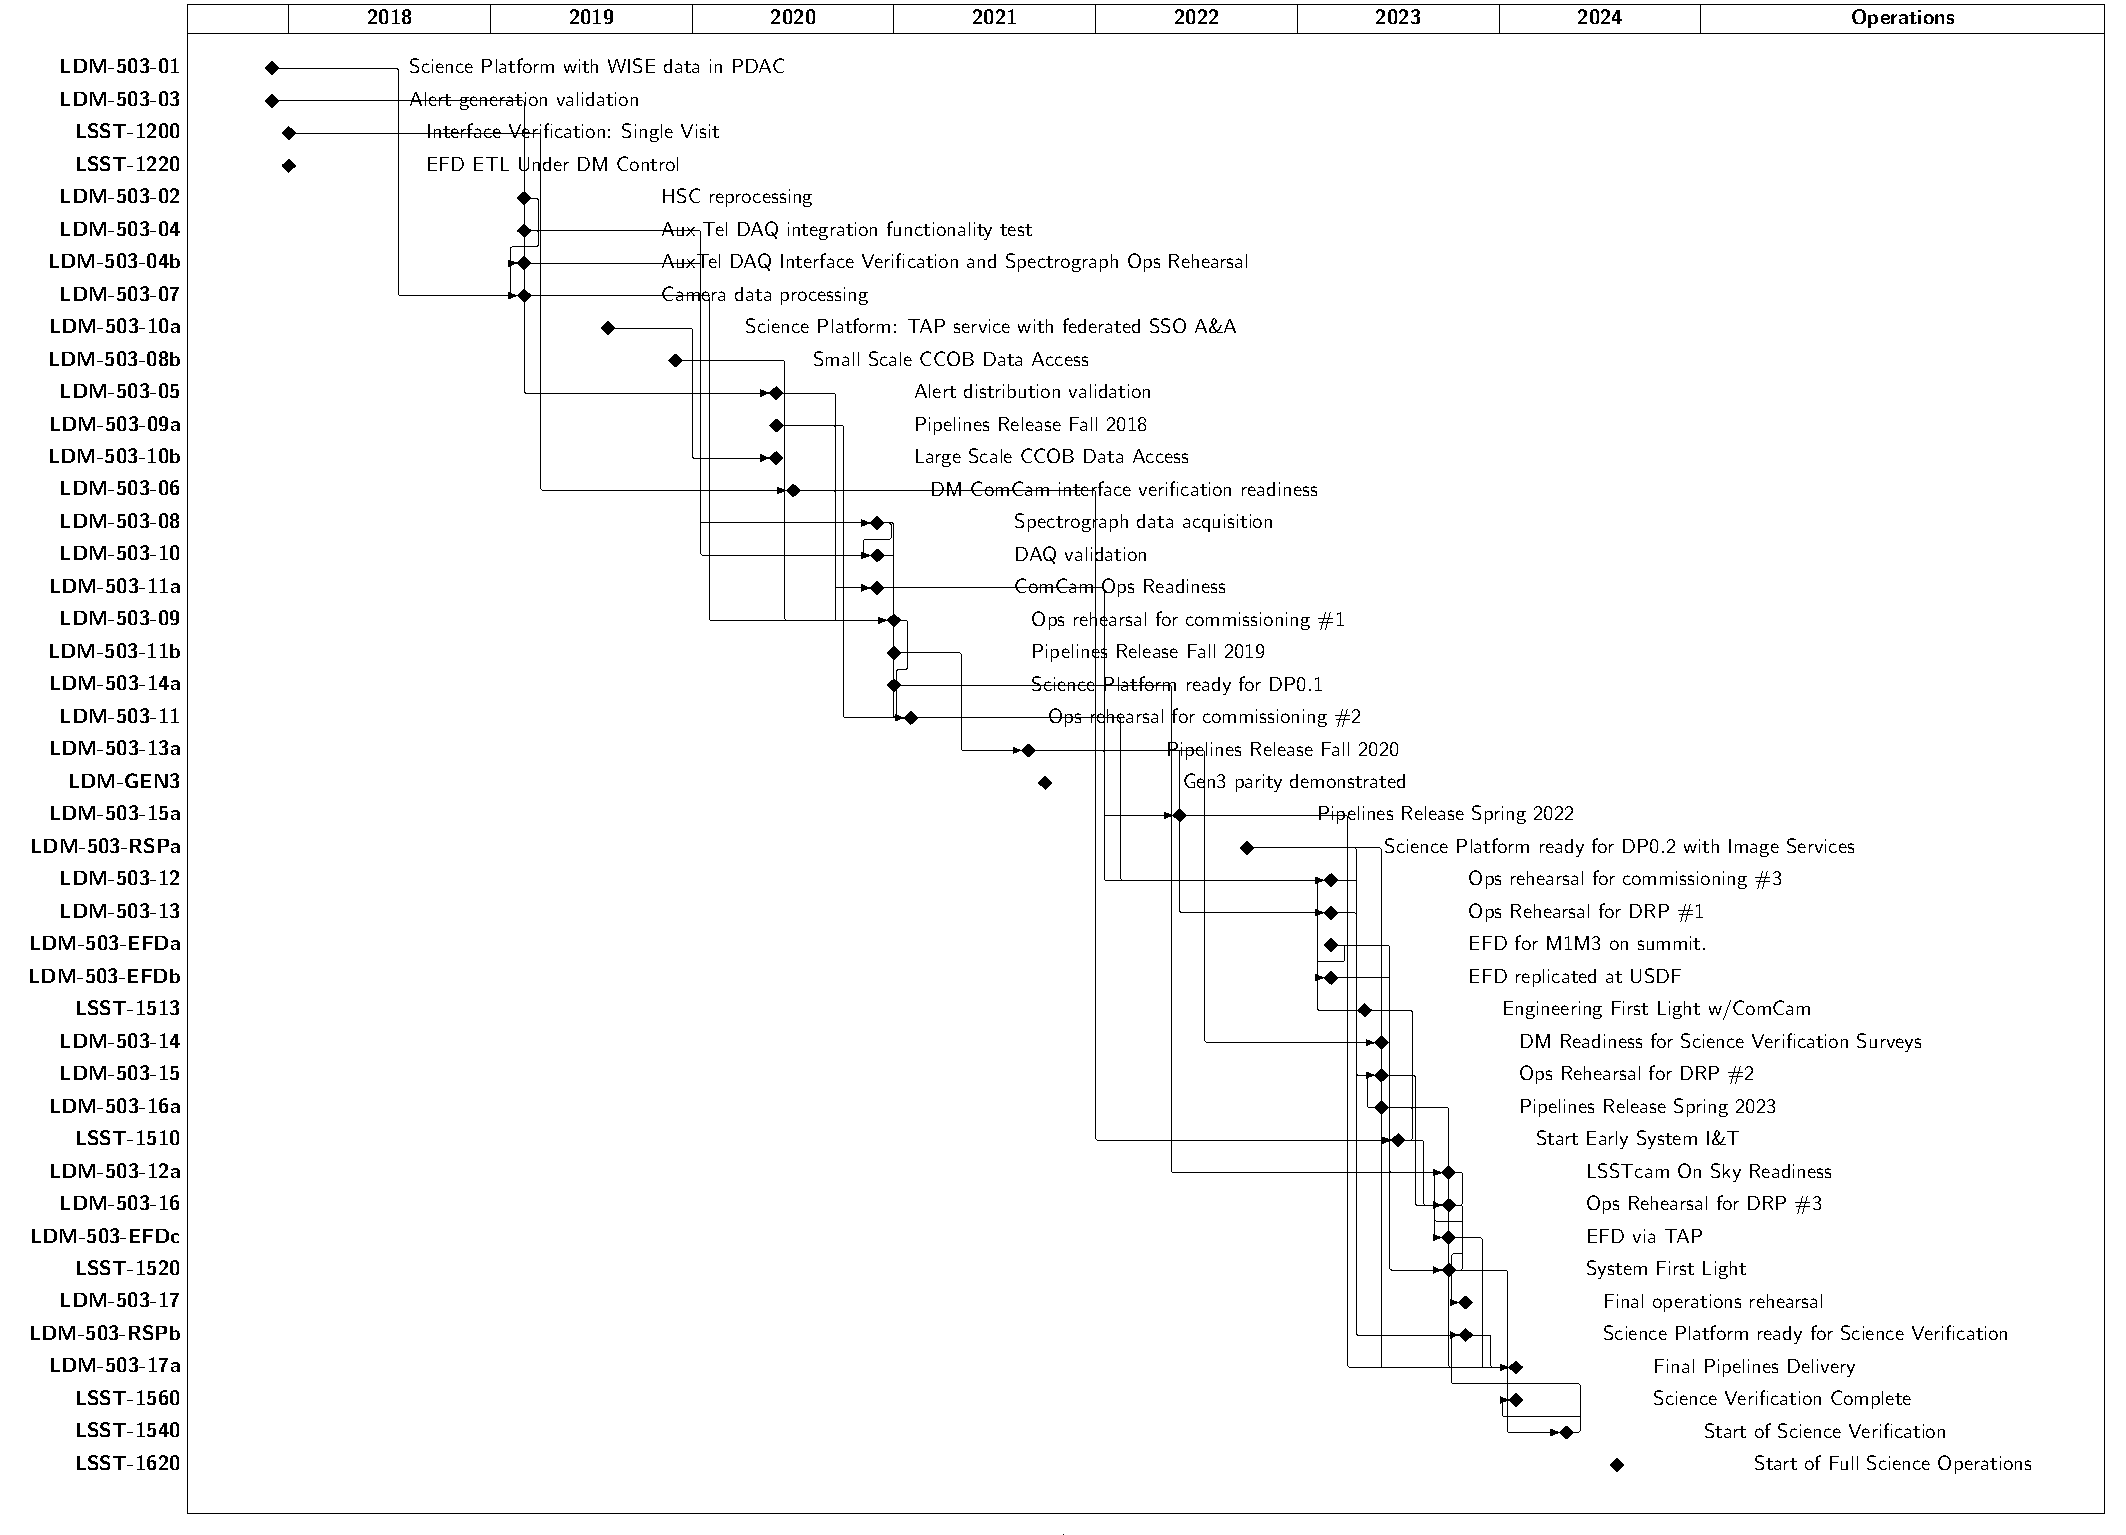
\includegraphics[width=\textwidth]{milestones/gantt}
		 \caption{DM major milestones---designated as LDM-503-\textit{x}---in
         the LSST schedule. These milestones are defined at level 2 according
         to the scheme described in \secref{sect:plan}.}
         \label{fig:schedule}
	 \end{center}
 \end{figure}

\subsection{Work breakdown structure}\label{sect:WBS}

While the original DM WBS is laid out in \citeds{LPM-43} with definitions provided in \citeds{LPM-44},
the new WBS is currently described in \appref{sec:wbslist}, which is expected to replace the contents of LPM-43 upon approval by the LSST CCB.

The WBS provides a hierarchical index of all hardware, software, services, and other deliverables which are required to complete the LSST Project.
It consists of alphanumeric strings separated by periods.
The first component is always “1”, referring to the LSST Construction Project.
``02C'' in the second component corresponds to Data Management Construction.
Subdivisions thereof are indicated by further digits.
These subdivisions correspond to teams within the DM project.
The top level WBS elements are mapped to the lead institutes in \tabref{tab:wbs}; the lead institutions roles are outlined in \secref{sect:leadtutes}.
The various groups involved in the WBS are briefly described in \secref{sect:groups}.

\begin{table}
\caption{DM top level Work Breakdown Structure \label{tab:wbs}}
\begin{center}
\begin{tabular}[htb]{|l|l|l|} \hline
\textbf{WBS}  &  \textbf{Description}   &  \textbf{Lead Institution}\\ \hline
1.02C.01& System Management                         &  LSST Tucson \\ \hline
1.02C.02& Systems Engineering                       &  LSST Tucson \\ \hline
1.02C.03& Alert Production                          &  University of Washington\\ \hline
1.02C.04& Data Release Production                   &  Princeton University\\ \hline
1.02C.05& Science User Interface and Tools          & IPAC\\ \hline
1.02C.06& Science Data Archive                      & SLAC\\ \hline
1.02C.07& LSST Data Facility                        & NCSA\\ \hline
1.02C.08& International Communications \& Base Site & LSST Tucson \\ \hline
1.02C.09& System Level Testing \& Science Validation& LSST Tucson \\ \hline
1.02C.10& Science Quality \& Reliability Engineering& LSST Tucson \\ \hline
\end{tabular}
\end{center}
\end{table}

\subsection{Planning Process}\label{sect:plan}

Milestones have been defined to describe the major goals of the DM subsystem throughout the construction project.
Each milestone has a description, a due date, and a level.
Four levels are defined:

\begin{description}
\item[Level 1]{The most important milestones exposed at the NSF level.}
\item[Level 2]{Cross-subsystem milestones (for example, DM milestones that affect the Camera Subsystem).}
\item[Level 3]{Cross-team milestones within DM (for example, Middleware milestones that affect the DRP Team).}
\item[Level 4]{Internal milestones within a team.}
\end{description}

The major DM subsystem tests described in \secref{sect:schedule} are defined as level 2 milestones.
Teams plan their work towards each test by defining a series of level 3 milestones.
Teams may define level 4 milestones for their own use.

Resources to achieve the milestones throughout the duration of construction have been allocated by means of \textit{planning packages} loaded into the PMCS.
Each top level WBS within DM (per \tabref{tab:wbs}) is divided into some tens of planning packages, each of which addresses some part of the DM baseline design with a clearly defined scope, deliverable, resource cost, and end date.

As the due date for work approaches, the actions required to complete each planning package---and hence meet the associated milestones---must be defined in detail.
The DM team divides the year into two six month long \textit{cycles}, running from November through May (the ``spring cycle'') and from June through October (the ``fall cycle'').
At the start of each cycle, the DM Leadership Team (\secref{sect:dmlt}) agrees on the detailed plan of work for the cycle, and this is loaded in to Jira as a series of ``epics'', corresponding to projects of a few person-months duration, each with defined start and end dates and resource loading.
The DM team records work and tracks progress against epics using Jira; the Project Controller (\secref{role:pcon}) arranges for this information to be ingested to and made available within the PMCS.
When epics are closed the T/CAM should ensure the deliverables are mentioned/linked in the associated comments in Jira. The DMPM shall verify all closed epics have the defined deliverables associated with them.

This process is described in detail in \citeds{DMTN-020}.

\section{Products \label{sect:products}}

The products of DM are not the data products defined in \citeds{LSE-163},
but rather the artifacts, systems, and services which will be used by the
operational LSST system to generate those data products.

In \secref{sect:dmarc}, we briefly described the high level approach being taken to the design of the DM products, while \appref{sect:prodlist} provides a complete list of products, including the technical manager, WBS element, and product owner for each.
That information is summarized in the product tree shown in \figref{fig:prods}.

Each DM product is being developed to satisfy one or more of the requirements placed upon the DM subsystem. \citeds{LDM-148} provides a tracing from each product to and from the relevant requirements.
These requirements are drawn from \citeds{LSE-61}, the DM System Requirements document.
The requirements \citeds{LSE-61} are themselves traced to higher level requirements in
the Observatory System Specifications (OSS; \citeds{LSE-30}) (See also \figref{fig:doctree}).
\appref{sect:tracefor} traces DM requirements to higher level requirements, and \appref{sect:traceback} traces relevant higher-level requirements to DM.

\begin{figure}[htbp]
	\begin{center}
		 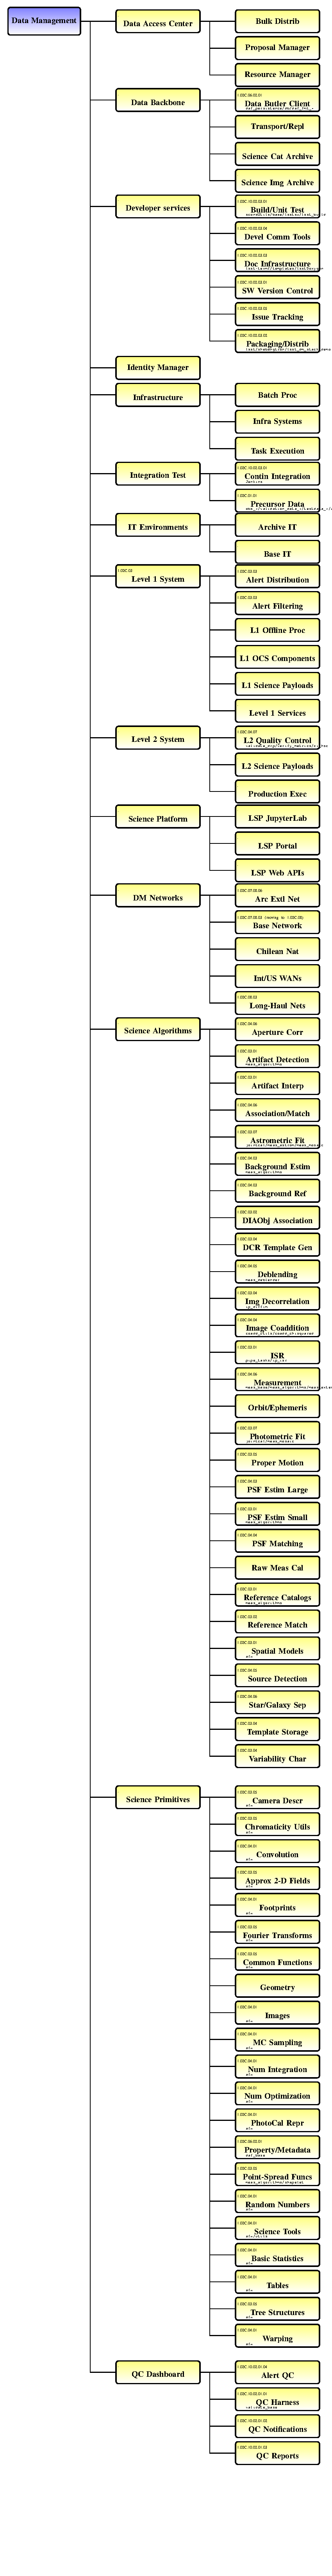
\includegraphics[height=19cm]{ProductTree}
         \caption{An overview of the DM product tree. This provides just a summary of the highest level items: refer to \appref{sect:prodlist} for the full list.}
         \label{fig:prods}
	 \end{center}
 \end{figure}

Every code repository used by DM must be associated with a product, and hence will have an associated technical manager and product owner.

\section{Roles in \gls{Data Management}}

This section describes the responsibilities associated with the roles shown in
\figref{fig:dmorg}.


\subsection{DM \gls{Project Manager} (\gls{DMPM})\label{role:dmpm}}

The \gls{DM} \gls{Project Manager} is responsible for the efficient coordination of all \gls{LSST} activities and responsibilities assigned to the \gls{Data Management} \gls{Subsystem}. The \gls{DM} \gls{Project Manager} has the responsibility of establishing the organization, resources, and work assignments to provide \gls{DM} solutions.  The \gls{DM} \gls{Project Manager} serves as the \gls{DM} representative in the \gls{LSST} Project Office and in that role is responsible for presenting \gls{DM} initiative status and submitting new \gls{DM} initiatives to be considered for approval. Ultimately, the \gls{DM} \gls{Project Manager}, in conjunction with his/her peer Project Managers (Telescope, \gls{Camera}), is responsible for delivering an integrated \gls{LSST} system. The \gls{DM} \gls{Project Manager} reports to the \gls{LSST} \gls{Project Manager}. Specific responsibilities include:

\begin{itemize}
\item Manage the overall \gls{DM} System
\item Define scope and request funding for \gls{DM} System
\item Develop and implement the \gls{DM} project management and control process, including earned value management
\item Approve the \gls{DM} \gls{Work Breakdown Structure} (\gls{WBS}), budgets and resource estimates
\item Approve or execute as appropriate all \gls{DM} outsourcing contracts
\item Convene and/or participate in all \gls{DM} reviews
\item Co-chair the \gls{DM} Leadership Team (\secref{sect:dmlt})
\end{itemize}

\subsection{Deputy DM \gls{Project Manager} (\gls{DDMPM}) \label{role:ddmpm}}
The PM and deputy will work together on the general management of DM and any specific PM tasks may be delegated to the deputy as needed and agreed. In the absence of the PM the deputy carries full authority and decision making powers of the PM. The DM Project Manager will keep the Deputy Project Manager informed of all DM situations such that the deputy may effectively act in place of the Project Manager when absent.

\subsection{DM \gls{Subsystem Scientist} (\gls{DMSS}) \label{role:dmps} }

The DM \gls{Subsystem Scientist} (\gls{DMSS}) has the ultimate responsibility for ensuring DM initiatives provide solutions that meet the overall \gls{LSST} science goals. As such, this person leads the definition and understanding of the science goals and deliverables of the \gls{LSST} \gls{Data Management} System and is accountable for communicating these to the DM engineering team.

The DM \gls{Subsystem Scientist} reports to the \gls{LSST} \gls{Project Scientist}. The \gls{DMSS} is a member of the \gls{LSST} \gls{Change Control Board} and the \gls{Project Science Team}. He/she chairs and directs the work of the DM System Science Team (\secref{sect:dmsst}).

Specific responsibilities and authorities include:


\begin{itemize}
\item Communicates with \gls{DM} science stakeholders (\gls{LSST} \gls{Project Scientist} and Team, advisory bodies, the science community) to understand their needs and identifies aspects to be satisfied by the \gls{DM} \gls{Subsystem}.
\item Develops, maintains, and articulates the vision of \gls{DM} products and services responsive to stakeholder needs.
\item Works with the \gls{LSST} \gls{Project Scientist} to communicate the \gls{DM} System vision to \gls{DM} stakeholders. Works with the \gls{DM} \gls{Project Manager} to communicate and articulate the \gls{DM} System vision and requirements to the \gls{DM} construction team.
\item Regularly monitors \gls{DM} construction team progress and provides feedback to the \gls{DM} \gls{Project Manager} to ensure the continual understanding of and adherence to the \gls{DM} vision, requirements, and priorities.
\item Develops and/or evaluates proposed changes to \gls{DM} deliverables driven by schedule, budget, or other constraints.
\item Provides advice to the \gls{DM} \gls{Project Manager} on science-driven prioritization of construction activities.
\item Validates the science quality of \gls{DM} deliverables and the capability of all elements of the \gls{DM} System to achieve \gls{LSST} science goals.
\item Serves as \gls{Data Management} Liaison as requested by \gls{LSST} Science Collaborations
\item Provides safe, effective, efficient operations in a respectful work environment.
\end{itemize}

Specific authorities include:

\begin{itemize}
\item Defines the vision and high-level requirements of the \gls{DM} products and services required to deliver on \gls{LSST} science goals.
\item Defines the science acceptance criteria for \gls{DM} deliverables (both final and intermediate) and validates that they have been met (Science \gls{Validation}).
\item Hires or appoints \gls{DM} System Science Team staff and other direct reports and defines their responsibilities.
\item Advises and consents to the appointments of institutional \gls{DM} Science Leads.
\item Delegates authority and responsibility as appropriate to institutional Science Leads and other members of the DM System Science Team.
\item Represents and speaks for the \gls{LSST} \gls{Data Management}.
\item Convenes and/or participates in all \gls{DM} reviews.
\item Co-Chairs the \gls{DM} Leadership Team
\end{itemize}

\subsection{Deputy DM \gls{Subsystem Scientist} (\gls{DMSS}) \label{role:ddmss} }

The relationship the \gls{Subsystem Scientist} and deputy is equivalent to that
between the \gls{Project Manager} and deputy (see \secref{role:ddmpm}).


\subsection{Project Controller/Scheduler \label{role:pcon}}

The \gls{DM} Project Controller is responsible for integrating \gls{DM}'s agile planning process with the \gls{LSST} Project Management and Control System (\gls{PMCS}). Specific responsibilities include:

\begin{itemize}

  \item{Assist T/CAMs in developing the \gls{DM} plan}
  \item{Synchronize the \gls{DM} plan, managed as per \secref{sect:plan}, with the \gls{LSST} PMCS}
  \item{Ensure that the plan is kept up-to-date and milestones are properly tracked}
  \item{Create reports, Gantt charts and figures as requested by the \gls{DMPM}}

\end{itemize}

\subsection{Product Owner \label{role:prodo}}

A product owner is responsible for the quality and acceptance of a particular product.
The product owner shall sign off on the requirements to be fulfilled in every delivery and therefore also on any descopes or enhancements.
The product owner shall define tests which can be run to prove a delivery meets the requirements due for that product.

\subsection{Senior advisor / Pipelines Scientist \label{role:pipe}}

The Senior advisor has direct communicaitons with the \gls{PM}. Several \gls{DM} products come together to form the \gls{LSST} \gls{pipeline}. The Pipelines Scientist is the product owner for the overall \gls{pipeline}.

The Pipelines Scientist shall:

\begin{itemize}

\item Provide guidance and test criteria for the full \gls{pipeline} including how \gls{QA} is done on the products
\item Keep the big picture of where the codes are going in view, predominantly with respect to the algorithms, but also the implementation and architecture (as part of the \gls{Systems Engineering} Team \secref{sect:sysengt}).
\item Advise on how we should attack algorithmic problems, providing continuing advice to subsystem product owners as we try new things.
\item Advise on \gls{calibration} issues, provide understanding of the detectors from a \gls{DM} point of view
\item Advise on the overall (scientific) performance of the system, and how we'll test it, thinking about all the small things that we have to get right to make the overall system good.

\end{itemize}

\subsection{Science Platform Scientist \label{role:scip}}
The science platform is composed of three aspects. Each aspect is produced in a different institution.
Each aspect has its own science lead/product owner.
The product owner for the platform is the \gls{DM} \gls{Subsystem Scientist} \secref{role:dmps} with final say on requirements and features, however since this is a vital tool for \gls{LSST} science we feel it is also important to have a scientist considering the platform as a whole.
Hence this role is to be the scientific guardian of the science platform as a whole, to make sure all of the aspects work together in a useful manner allowing scientific exploitation of the \gls{LSST} data. The \gls{Science Platform} Scientist works in close collaboration with the \gls{DM} \gls{Subsystem Scientist}.

\subsection{Systems Engineer \label{role:sysengineer}}

With the \gls{Systems Engineering} Team (\secref{sect:sysengt}) the \gls{Systems Engineer} owns the \gls{DM} entries in the risk register and is generally in charge of the \textit{process} of building \gls{DM} products.

As such, the \gls{Systems Engineer} is responsible for managing requirements as they pertain to \gls{DM}.
This includes:

\begin{itemize}
\item Update and ensure traceability of the high level design \& requirements documents: \gls{DMSR} (\citeds{LSE-61}), \gls{OSS} (\citeds{LSE-30}), and \gls{LSR} (\citeds{LSE-29})
\item Oversee work on lower level requirements documents
\item Ensure  that the system is appropriately modeled in terms of e.g. drawings, design documentation, etc
\item Ensure  that solid verification plans and standards are established within \gls{DM}
\end{itemize}

In addition, the \gls{Systems Engineer} is responsible for the process to define \& maintain \gls{DM} interfaces (internal and external)

\begin{itemize}
\item Define and enforce standards for internal interfaces
\item Direct the Interface Scientist's (\secref{role:dmis}) work on external ICDs
\end{itemize}

The \gls{Systems Engineer} shall chair the \gls{DM} \gls{Change Control Board} (\secref{sect:dmccb})

\begin{itemize}
\item Organize \gls{DMCCB} processes so that the change control process runs smoothly
\item Identify RFCs requiring \gls{DMCCB} attention
\item Shepherd RFCs through change control
\item Call and chair \gls{DMCCB} meetings, ensuring that decisions are made and recorded
\end{itemize}

Finally, the \gls{Systems Engineer} represents \gls{DM} on the \gls{LSST} \gls{CCB}.

\subsection{DM Interface Scientist (\gls{DMIS}) \label{role:dmis}}

The \gls{DM} Interface Scientist is responsible for all external interfaces to the \gls{DM} \gls{Subsystem}. This includes ensuring that appropriate tests for those interfaces are defined. This is a responsibility delegated from the \gls{DM} \gls{Systems Engineer} (\secref{role:sysengineer}).

As we begin to implement these interfaces this role will diminish as implementers take up the ownership of the interfaces.

\subsection{Software Architect \label{role:softarc}}

The Software Architect is responsible for the overall design of the \gls{DM} \textit{software} system. Specific responsibilities include:

\begin{itemize}

\item{Define the overall architecture of the system and ensuring that all products integrate to form a coherent whole}
\item{Select and advocate appropriate software engineering techniques}
\item{Choose the technologies which are used within the codebase}
\item{Minimize the exposure of \gls{DM} to volatile external dependencies}

\end{itemize}

The Software Architect will work closely with the \gls{Systems Engineer} (\secref{role:sysengineer}) to ensure that processes are in place for tracing requirements to the codebase and providing hooks to ensure that requirement verification is possible.

\subsection{Operations Architect \label{role:opsarc}}

The \gls{DM} \gls{Operations} Architect is responsible for ensuring that all elements of the \gls{DM} \gls{Subsystem}, including operations teams, infrastructure, middleware, applications, and interfaces,
come together to form an operable system.

Specific responsibilities include:

\begin{itemize}
\item Set up and coordinate operations rehearsals
\item Ensure readiness of procedures and personnel for \gls{Operations}
\item Set standards for operations e.g. procedure handling and operator logging
\item Participate in stakeholder and end user coordination and approval processes and reviews
\item Serve as a member of the \gls{LSST} \gls{Systems Engineering} Team
\end{itemize}

\subsection{Release Manager (\gls{RM})}\label{role:dmrm}

The \gls{DM} \gls{Release} Manager (\gls{RM}) is responsible for maintaining and applying the release policy.
Specifically, the \gls{DM} \gls{Release} Manager will:

\begin{itemize}

  \item{Develop and maintain the \gls{DM} \gls{Release} Policy as a change controlled
  document;}
  \item{Manage the software release process and its compliance with documented
  policy;}
  \item{Define the contents of releases, in conjunction with the product
  owners, the \gls{DM} \gls{Subsystem Scientist}, and the technical managers;}
  \item{Ensure that each release is accompanied by an appropriate
  documentation pack, including user manuals, test specifications and reports,
  and release notes;}
  \item{Ensure the release is delivered to \gls{NCSA} for acceptance;}
  \item{Work with technical managers to coordinate bug fixes and maintenance
  of long-term support releases;}
  \item{Serve as a member of the \gls{DMCCB} (\secref{sect:dmccb}).}

\end{itemize}

\subsection{Lead Institution Senior Positions}

Each Lead Institution (as defined in \secref{sect:leadtutes}; see also \tabref{tab:wbs}) has a \gls{T/CAM} and Scientific or Engineering Lead, who jointly have overall responsibility for a broad area of \gls{DM} work, typically a \gls{Work Breakdown Structure} (\gls{WBS}) Level 2 element. They are supervisors of the team at their institution, with roles broadly analogous to those of the \gls{DM} \gls{Project Manager} and \gls{Subsystem Scientist}.

\subsubsection{Technical/Control Account Manager (\gls{T/CAM}) \label{role:tcam}}

Technical/Control Account Managers have managerial and financial responsibility
for the engineering teams within \gls{DM}. Each \gls{T/CAM} is responsible for a specific set of \gls{WBS} elements. Their detailed responsibilities include:

\begin{itemize}

  \item{Develop, resource load, and maintain the plan for executing the \gls{DM} construction project within the scope of their WBS}
  \item{Synchronize the construction schedule with development in \gls{WBS} elements managed by other T/CAMs}
  \item{Maintain the budget for their \gls{WBS} and ensuring that all work undertaken is charged to the correct accounts}
  \item{Work with the relevant Science Leads and Product Owners (\secref{role:prodo}) to develop the detailed plan for each cycle and sprint as required}
  \item{Work with the \gls{DM} Project Controller (\secref{role:pcon}) to ensure that all plans and milestones are captured in the \gls{LSST} Project Controls system}
  \item{Perform day-to-day management of staff within their \gls{WBS}}
  \item{Perform the role of ``scrum-master'' during agile development}
  \item{Report activities as required, including providing input for monthly status reports.}

\end{itemize}

\subsubsection{Institutional Science/Engineering Lead \label{role:scilead}}

The Institutional Science/Engineering Leads serve as product owners (\secref{role:prodo}) for the major components of the \gls{DM} System (\gls{Alert Production}, Data \gls{Release} Production, Science User Interface etc).

In addition, they provide scientific and technical expertise to their local engineering teams.

They work with the \gls{T/CAM} who has managerial responsibility for their product to define the overall construction plan and the detailed cycle plans for \gls{DM}.

Institutional science leads are members of the \gls{DM} System Science Team (\secref{sect:dmsst}) and, as such, report to the \gls{DM} \gls{Subsystem Scientist} (\secref{role:dmps}).

\subsection{DM Science \gls{Validation} Scientist}
\label{role:dmsvs}

The \gls{DM} Science \gls{Validation} Scientist leads the Science \gls{Validation} team (\secref{sect:dmsvt}).
This individual has primary responsibility for planning, executing and analyzing the results of science validation activities, as defined in \citeds{LDM-503}; typically, this includes large-scale data challenges.
The Science \gls{Validation} Scientist is responsible for End to End Science validation and reports to the \gls{DM} \gls{Subsystem Scientist}.

\subsection{Cross-Cutting Roles}\label{role:crosscut}

There are at least two roles which involve managing work across institute and \gls{WBS} boundaries.
These individuals act as coordinators for the cross-cutting activity, including organizing ``standup'' (or other) meetings and resolving technical difficulties.
They should develop a master schedule for activities within their area of responsibility and synchronize it with the T/CAMs who are managing individual teams.
Day-to-day management of staff resides with the \gls{T/CAM} of the appropriate \gls{WBS}; it follows that stories can only be assigned to individuals with the agreement of that \gls{T/CAM}.
Though this is more of a coordination-oriented role, these managers have authority to prioritize stories in the relevant area.

\subsubsection{Science Platform Manager}\label{role:lsplead}

The \gls{LSST} \gls{Science Platform} spans multiple \gls{WBS} elements bringing together authentication, front-end services, database access, and notebook execution.
At time of writing, Frossie Economou is the \gls{Science Platform} Manager.

\subsubsection{Middleware Manager}\label{role:mwlead}

Middleware covers several \gls{WBS} elements and requires multiple parts of the system to work in unison.
This includes task execution, workflow management, data access abstractions (the ``Data \gls{Butler}''), and \gls{provenance}.
At time of writing, Fritz Mueller is the Middleware Manager.

\section{Teams within Data Management} \label{sect:groups}

Since the DM team is distributed in terms of geography and responsibility across the Rubin partner and lead institutions, mechanisms are needed to ensure that the project remains on track at all times. There are five primary coordinating bodies to ensure the management, technical, and quality integrity of the DM Subsystem.

\subsection{System Science Team \label{sect:dmsst}}

Members of the DM System Science Team (SST) work together to define, maintain, and communicate to the DM Systems Engineering team a coherent vision of the Rubin DM system responsive to the overall Rubin Project goals, as well as scientifically validate the as-built system (\citeds{LDM-503}, Section~9.).

\begin{figure}[htbp]
\begin{center}
\includegraphics[width=0.8\textwidth]{images/DmSSTOrg}
\caption{DM System Science Team organisation.
\label{fig:sstorg}}
\end{center}
\end{figure}



\subsubsection{Organization and Goals}
\label{sect:dm-sst-org}

The System Science Team includes:
\begin{itemize}
\item \gls{DMSS} (chair)
\item DM Science Validation Scientist
\item DM Institutional Science Leads
\item DM System Science Analysts
\item DM Science Pipelines Scientist
\end{itemize}

The System Science Team has been chartered to:
\begin{itemize}
\item Support the \gls{DMSS} (as the overall DM Product Owner) in ensuring that Data Management Subsystem's initiatives provide solutions that meet the overall Rubin science goals.
\item Support the Institutional Science Leads in their roles as Product Owners for elements of the DM system their respective institutions have been tasked to deliver.
\item Support the DM Science Validation Scientist, who organizes and coordinates the science validation efforts (\citeds{LDM-503}).
\item Guide the work of System Science Analysts, who generally lead and/or execute studies needed to support SST work.
\item Provide a venue for communication with the Science Pipelines Scientist, who broadly advises on topics related to the impact of science pipelines on delivered science and vice versa (\secref{role:pipe}).
\end{itemize}

The members of the System Science Team report to the \gls{DMSS} and share the following responsibilities:
\begin{itemize}
\item Communicate with the science community and internal stakeholders to understand their needs, identifying the aspects to be satisfied by the DM Subsystem.
\item Liaise with the science collaborations to understand and coordinate any concurrent science investigations relevant to the DM Subsystem.
\item Develop, maintain, and articulate the vision of DM-delivered LSST data products and services that is responsive to stakeholder needs, balanced across science areas, well motivated, and scientifically and technologically current.
\item Work with the \gls{DMPM} and DM \glspl{T/CAM} to communicate and articulate the DM System vision and requirements to the DM engineering team.
\item Identify, develop, and champion new scientific opportunities for the Rubin DM System, as well as identify risks where possible.
\item Develop change proposals and/or evaluate the scientific impact of proposed changes to DM deliverables driven by schedule, budget, or other constraints.
\item Lead the Science Verification of the deliverables of the DM subsystem.
\end{itemize}

\subsubsection{Regression Monitoring of KPMs and other Metrics}

All KPMs and other regression monitoring metrics will be calculated on a regular cadence (daily if possible).
They are monitored by the SQuaRE scientist, with status periodically reported to the System Science Team (SST).
The SQuaRE scientist brings up any major regressions to the attention of the SST, along with an initial assessment of the problem.
The SST has the responsibility of monitoring the overall system for whether it meets its key performance metrics as well as understanding any significant performance regressions in performance.
The SST may recommend further actions to the \gls{DMPM} and/or \gls{DMSS}, if necessary.
These include performing additional testing, broader root cause analysis, documenting the regression, or recommendations on the priority of fixing the regression relative to presently scheduled work.

\subsubsection{Communications}

DM System Science Team communication mechanisms are described on the SST Confluence page at \url{http://ls.st/sst}. The list of current  DM liaisons to the LSST Science Collaborations and international partners is maintained  in  \url{https://www.lsstcorporation.org/science-collaborations}

\subsubsection{Time Allocation for Institutional Science Leads}

The Institutional Science Leads fulfill the role of \textit{Product Owner} for elements of the DM system that their respective institutions have been tasked to deliver; institutional T/CAMs rely on their Scientist to provide  \emph{Product Owner}  services.
In addition, as members of the DM System Science Team, they have responsibilities as described in \ref{sect:dm-sst-org}, which result in work that is more \textit{emergent} in nature.
To balance these two roles, the \gls{DMSS} is entitled to allocate up to 50\% of the Institutional Science Leads' time to Science Team work.
If any Science Team study should require a greater commitment, additional time must be negotiated and agreed with the institutional \glspl{T/CAM}s.
This arrangement is intended to ensure both a good working relationship between the T/CAMs and scientists, and that the \gls{DMSS} maintains sufficient support from the Science Team to deliver a system that meets the overall Rubin science goals.

\subsection{DM Systems Engineering Team \label{sect:sysengt}}

The Systems Engineering Team is led by the DMPM (\secref{role:dmpm}) and looks after all aspects of systems engineering.
It is comprised of not only the Systems Engineer (\secref{role:sysengineer}), but also the Software Architect (\secref{role:softarc}), Operations Architect (\secref{role:opsarc}), \gls{DMSS} (\secref{role:dmps}), Pipeline Scientist (\secref{role:pipe}), Interface Scientist (\secref{role:dmis}), and the \gls{DDMPM} (\secref{role:ddmpm}).

While the product owners (\secref{role:prodo}) help DM to create products which are fit for purpose, the Systems Engineering Team must ensure we do it correctly. This group concerns itself with (sub)system wide decisions on architecture and software engineering.

The specific tasks of this group include:

\begin{itemize}
\item Formalize the product list for DM\footnote{In this sense, ``products'' are the software and systems which produce data products, rather than the data products themselves. See also \ref{sect:products}.}
\item Formalize the documentation tree for DM, defining which documents need to be produced for each product
\item Agree the process for tracing the baseline requirements verification and validation status.
\item Agree the formal versions of documents and software which form the technical baseline, individual items will go through the CCB for formal approval.  This includes upload to docushare.
\item Perform releases of software products --- including, but not limited to, the Science Pipelines --- as needed, using tooling provided by SQuaRE (\secref{sect:square}).
\item Debug unexpected build problems:
\begin{itemize}
  \item{Resolve issues related to the underlying build infrastructure directly;}
  \item{Pass off product-specific problems to the relevant product team.}
\end{itemize}
\item Maintain the build/packaging system e.g.  newinstall.sh, lsstsw, lsst\_build and EUPS.
\end{itemize}

Some of these tasks are will be delegated to individual group members.
These individuals also are the conduit to/from the rest of the DM team to raise ideas/issues with the engineering approach.

\subsubsection{Communications}

The Systems Engineering Team will only physically meet to discuss specific topics: there will not be a regular meeting of the group outside of the one to one meetings with the DM project manager for the individuals in the group.
Discussions will be held via email until in person talks are required.


\subsection{Chile IT Team \label{sect:chit}}
The Chile IT lead (Cristían Silva) has responsibility for the IT infrastructure in Chile. This includes the \gls{LHN}.
For more details on Chile IT see \citeds{ITTN-006}.
A brief set of responsibilities include:
\begin{itemize}
\item Provide desktop support for Chile users at the base, Tucson Labs, and summit.
\item Handle all IT hardware and software purchases in Chile.
\item Handle all IT installations in Chile.
\item Handle Long Haul Network contracts and meetings.
\item Provide infrastructure as code layer (Puppet/Kubernetes etc.) upon which other teams may deploy services.
\item Provide networking for all the components of the observatory.
\item Provide monitoring of IT services
\item Provide authentication and authorization services for the operational facilities.
\item Provide video conferencing support
\item Provide backup facilities and ensure backups are made
\item Deployment and management of all layer 1 network connections in Rubin scope, including camera fibers, dome network, etc.
\end{itemize}

\subsubsection{Communications}
The IT lead must interact with other CAMS to ensure all services are provided as needed and agreed.
This means having representation at key telescope and site planning meetings (as well DMLT).
Chile IT lead will have a weekly tag up with IT Tucson and the DMPM.
Internally the team holds weekly and daily standups.

\subsection{DM Leadership Team \label{sect:dmlt}}

The purpose of the DM Leadership Team (DMLT) is to assist the DMPM  establish the scope of work and resource allocation across DM and ensure overall project management integrity across DM.
The following mandate established the DMLT:

\begin{itemize}
\item Charter/purpose
	\begin{itemize}
	\item Maintain scope of work and keep within resource allocation across DM
	\item Ensure overall project management integrity across DM
	\item Ensure Earned Value management requirements are met
	\end{itemize}
\item Membership
	\begin{itemize}
	\item Co-chaired by the \gls{DMPM} (\secref{role:dmpm}) and \gls{DMSS} (\secref{role:dmps})
	\item Lead Institution Technical/Control Account Managers (T/CAMs; \secref{role:tcam})
	\item Institutional Science or Engineering Leads (\secref{role:scilead})
	\item Members of the DM Systems Engineering Team (\secref{sect:sysengt})
	\end{itemize}
\item Responsibilities
	\begin{itemize}
	\item Prepares all budgets, schedules, plans
	\item Meets every week to track progress, address issues/risks, adjust work assignments and schedules, and disseminate/discuss general PM communications
	\end{itemize}
\end{itemize}

The DM Leadership Team and the DM Systems Engineering Team (\secref{sect:sysengt}) work in synchrony.
The DMLT makes sure the requirements and architecture/design are estimated and scheduled in accordance with Rubin Project required budgets and schedules.

 02C.08 LHN is a bit of an anomaly in the DM WBS and probably should not have been in the WBS. IT have recently been put in charge of this but project do not wish to restructure the WBS. As such  02C.08 remains in DM but the CAM is not considered part of DMLT (though welcome to attend).

 \subsubsection{Communications}
A mailing list\footnote{\url{lsst-dmlt@listserv.lsstcorp.org}} exists for DMLT related messages.
On Mondays the DMLT hold a brief (30 to 45 minutes) telecon. This serves to:

\begin{itemize}
\item Allow the Project manager and DM Scientist  to pass on important project level information and general guidance.
\item Raise any blocking or priority issues across DM --- this may result in calling a splinter meeting to further discuss with relevant parties.
\item Inform all team members of any change requests (LCRs) in process at Rubin level which may be of interest to or have an impact on DM
\item Check on outstanding actions on DMLT members
\end{itemize}

Face to Face meetings of DM are held twice a year\footnote{One of these has been virtual since late 2018 and with COVID-19 its not obvious we will return soon to in person meetings.}; these are opportunities to:

\begin{itemize}
\item Discuss detailed planning for the next cycle
\item Discuss technical topics in a face to face environment
\item Work together on critical issues
\item Help make DM function as a team
\end{itemize}

\subsection{DM Change Control Board \label{sect:dmccb}}

The DMCCB has responsibility for issues similar to those of the Rubin Change Control Board, but focused on the DM Subsystem.
The DMCCB reviews and approves changes to all baselines in the Subsystem, including proposed changes to the DM System Requirements (DMSR), reference design, sizing model, i.e. any LDM-series document.
The Technical Baseline, including software/hardware and documentation, is produced by DM and controlled by the DMCCB.
DMCCB validates that the form and content of the Technical Baseline is consistent with Rubin project standards such as the Systems Engineering Management Plan (SEMP) \citeds{LSE-17}.

\begin{itemize}
\item Responsibilities:
        \begin{itemize}
        \item Determine when deliverables (controlled documents and software) are ready to be baselined (placed under configuration controlled status) or released. This include LDM series documents.
        \item Review and approve/reject proposed changes to baselined items - any LCR must go through the DMCCB before being submitted to the project CCB.
        \item Review all RFCs and approves \textit{flagged} RFCs prior to 'Adoption'
        \item Monitor and approve DM software releases
        \item Monitor the status of issues in the DM project on Jira
        \item Ensure that the DM Technical Baseline (LDM-xxx) follows Rubin and DM configuration control processes.
        \end{itemize}
\item Membership:
        \begin{itemize}
        \item Core members:
                \begin{itemize}
                \item \gls{DMPM}
                \item \gls{DMSS}
                \item Systems Engineer, Chair (\secref{role:sysengineer}).
                \item Operations Architect
                \item Software Architect
                \item Release Manager, Secretary
                \end{itemize}
        \item Optional members (required when topics to discuss are relevant to their areas of expertise):
                \begin{itemize}
                \item Deputy \gls{DMSS}, when \gls{DMSS} is not available
                \item Pipeline Scientist
		\item Science Pipelines Architect (this aligns with an operational role)%Jim Bosch
                \item \glspl{T/CAM}, who can delegate as needed
                \end{itemize}
	\item For on-line virtual meetings, if a consensus or quorum is not reached within one week, the \gls{DMPM} will make a unilateral decision
        \item \gls{DMPM} can also make unilateral decisions in cases of urgency. In that case DMCCB will assess the change \textit{a posteriori}.
	\end{itemize}
\end{itemize}

The DMCCB will meet, physically or virtually, every week for 30 minutes. Agenda will be available beforehand.
Urgent decisions can be taken offline, outside the weekly meeting, in a modality to be defined by the DMCCB itself (email or slack channel).

All RFCs that implies one of the following changes:

\begin{itemize}
\item Changes to controlled documents
\item API changes to the codebase, including deprecation
\item Data model changes
\end{itemize}

need to be \textit{flagged} and therefore approved by the DMCCB, as detailed in the \href{https://developer.lsst.io/communications/rfc.html#rfc-exceptions}{Developer Guide}.


\subsection{DM Science Validation Team}
\label{sect:dmsvt}

The DM Science Validation Team guides the definition of, and receives the products of, science validation and dress rehearsal activities, following the long-term roadmap described in \citeds{LDM-503}.
Decisions on the strategic goals of these activities are made in conjunction with the \gls{DMSS} and \gls{DMPM}.

The DM Science Validation Team is chaired by the DM Science Validation Scientist (\secref{role:dmsvs}).
Its membership includes the DM Pipelines Scientist (\secref{role:pipe}) and the various Institutional Science/Engineering Leads (\secref{role:scilead}).
Depending on the activities currently being executed, other members of the System Science Team (\secref{sect:dmsst}), the wider DM Construction Project, and/or external experts may be temporarily added to the team.


\subsection{Middleware Team \label{sec:middleware}}

The Middleware Team is responsible for delivering the Data Butler and pipe\_base task framework, including supporting infrastructure to make it possible to deploy them at-scale in the Data Facility in support of Alert and Data Release Production pipeline execution.

The Middleware Team has a Product Owner (Robert Gruendl, NCSA at time of writing) and Manager (\secref{role:mwlead}).
However, it does not have a permanent staff; rather it draws on effort from across the Alert Production (\secref{sect:ap}), Data Release Production (\secref{sect:drp}), Data Access Services (\secref{sect:dax}), and Data Facility (\secref{sect:ldf}) groups, as well as other members of the subsystem as necessary.
Effort allocation is agreed between the Middleware Manager and the T/CAMs of the various institutes.

\subsection{Science Platform Team \label{sec:sciplat}}

The Science Platform Team is responsible for delivering the three aspects of the Rubin Science Platform, as described in \citeds{LDM-542}.

The Product Owner for the Science Platform is the \gls{DMSS}, supported by the Science Platform Scientist (\secref{role:scip}).
The team is managed by the Science Platform Manager (\secref{role:lsplead}).
They coordinate effort across the subsystem, drawing primarily on the Data Access Services (\secref{sect:dax}), Data Facility (\secref{sect:ldf}) and SQuaRE (\secref{sect:square}) teams.

\section{Lead institutions in \gls{DM} \label{sect:leadtutes}}

\subsection{LSST Tucson\label{sect:tucson}}

The \gls{LSST} Project Office in Tucson hosts the \gls{DMPM} (\secref{role:dmpm}), the \gls{DMSS} (\secref{role:dmps}), and the \gls{Systems Engineer} (\secref{role:sysengineer}).
In addition, it is home to the Science Quality and Reliability Engineering (\gls{SQuaRE}) group and \gls{LSST} International Communications and Base Site (\gls{ICBS}) groups, described below.

\subsubsection{Science Quality and Reliability Engineering \label{sect:square}}

The \gls{SQuaRE} group is primarily charged with providing technical feedback to the \gls{DMPM} that demonstrates that \gls{DM} is fulfilling its responsibilities with regard to quality — of both scientific data products and software — software performance, and reliability. As such, areas of activity include:

\begin{itemize}

\item Development of algorithms to detect and analyze quality issues with data\footnote{This may overlap with work carried out by the \gls{Science Pipelines} groups (\S\S\ref{sect:ap} \& \ref{sect:drp}). In some instances this will involve sharing code; in others, it may merit duplicating a \gls{metric} to ensure that it is correct.}

\item Infrastructure development to support the generation, collection, and analysis of data quality and performance metrics

\item \gls{DM} developer support services to ensure \gls{DM} is using appropriate tools to aid software quality

\item \gls{DM} documentation support, to include defining standards and providing tooling for documentation as well as some document writing

\item Development and support of the build infrastructure (e.g. Jenkins,  groovy and dm-jenkins-jobs ) and release tools (e.g. container creation) for all \gls{DM} software products

\item Deploy, host and manage repositories of release artifacts, such as private Conda repositories, to support releases as needed and agreed with the Systems Engineering Team (\secref{sect:sysengt})

\end{itemize}

In the event that \gls{SQuaRE} identifies issues with the performance or future maintainability of the \gls{DM} codebase, it will bring them to the attention of the \gls{DM} Software Architect. In the event that \gls{SQuaRE} identifies issues with the quality of the data or algorithmic performance, it will bring them to the attention of the \gls{DMSS}.

\subsubsection{LSST International Communications and Base Site}
The \gls{ICBS} group spans both Tucson and La Serena, and is responsible for the design, procurement, installation, deployment, verification, and operating support during construction and commissioning of all data communications networks at the \gls{Summit} and Base sites, as well as links between all the \gls{LSST} Sites, with two exceptions:  the \gls{Summit} Network (\gls{WBS} 1.04C.12.5) and the \gls{Archive} External Network (1.02C.07.04.06).  In the case of the exceptions, there are technical and managerial interfaces between the \gls{ICBS} and the responsible parties, as well as overlaps of staff.  The \gls{LSST} Network Engineering Team (\gls{NET}) spans all of these networking assignees and is chaired by the \gls{ICBS} staff.

The \gls{ICBS} group is also jointly responsible with the Data Facility Team at \gls{NCSA} for procurement, installation, deployment, verification, and operating support during construction and commissioning of the computing and storage infrastructure at the Base Site.

Since a large majority of the \gls{ICBS} work involves procurement and contracted services, the group works in close cooperation with \gls{AURA} procurement and contracts, as well as with the following major sub-awardees and their subcontractors:

\begin{itemize}
	\item \gls{REUNA}: Chilean National Networks
	\item Florida International University/AmLight: International Networks connecting Chile and the United States, and \gls{US} National Networks.
\end{itemize}

\subsection {Princeton University \label{sect:princeton}}

Princeton University hosts the Pipelines Scientist (\secref{role:pipe}) and the \gls{DRP} group, described below.

\subsubsection{Data Release Production \label{sect:drp}}

The \gls{DRP} group has three major areas of activity within \gls{DM}.

\begin{itemize}

  \item{Definition and implementation of the scientific algorithms and pipelines which will be used to generate \gls{LSST}'s annual data releases;}

  \item{Definition and implementation of the algorithms and pipelines which will be used to produce the ``calibration products'' (for example, flat fields, characterization of detector effects, etc) which will be used as inputs to the photometric \gls{calibration} procedure in both nightly and annual data processing. This includes the development of the spectrophotometric data reduction \gls{pipeline} for the Auxiliary Telescope;}

  \item{Development, in conjunction with the \gls{Alert Production} team (\gls{AP}; \secref{sect:ap}), of a library of re-usable software libraries and components which form the basis of both the \gls{AP} and \gls{DRP} pipelines and which are made available to science users within the \gls{LSST} \gls{Science Platform}.}

\end{itemize}

Development of software in support of annual data releases and of reusable software components are carried out under the direction of the \gls{DRP} Science Lead, who acts as product owner for this part of the system.
The \gls{DRP} Science Lead is ultimately responsible to both the Pipelines Scientist (\secref{role:pipe}) and \gls{DMSS} (\secref{role:dmps}).

The product owner for the \gls{calibration} products is the \gls{LSST} \gls{Calibration Scientist} (who doubles as the Pipelines Scientist, \secref{role:pipe}).
The \gls{Calibration Scientist} liaises with other \gls{LSST} subsystems and with the products owners of the annual and nightly data processing pipelines to ensure that appropriate \gls{calibration} products are available to those pipelines to enable them to meet specifications.

Management of the group is the responsibility of the Deputy \gls{Science Pipelines} \gls{T/CAM}, reporting to the \gls{Science Pipelines} \gls{T/CAM} and ultimately to the \gls{DMPM} (\secref{role:dmpm}).

The \gls{DRP} group is responsible for delivering software which adheres to the architectural and testing standard defined by the Software Architect (\secref{role:softarc}).
In addition, the \gls{DRP} group is responsible for testing each major product delivered to demonstrate its fitness for purpose, and working with the \gls{DMSS} and \gls{DM} System Science Team (\secref{sect:dmsst}) to define, run and analyze ``data challenges'' and other large scale tests to validate the performance of the data release production system.

\subsection {The University of Washington\label{sect:uw}}

Princeton University hosts the \gls{DDMPM} and Deputy \gls{DMSS} as well as the \gls{AP} group, described below.

\subsubsection{Alert Production\label{sect:ap}}

The \gls{AP} group has 4 major areas of activity within \gls{DM}.

\begin{itemize}

  \item{Definition and implementation of the scientific algorithms and pipelines which will be used to generate alerts from \gls{LSST}'s image stream.  This will serve as the alert generation \gls{pipeline};}

  \item{Definition and implementation a scalable and reliable system for transmitting the alerts generated by the alert generation \gls{pipeline} including a mechanism for applying simple filters to the stream. This is the alert distribution and filtering system;}

  \item{Definition and implementation of a system for identifying moving objects in our solar system and fitting their physical properties. This is the Moving Objects Processing System (\gls{MOPS});}

  \item{Development, in conjunction with the Data \gls{Release} Production team (\gls{DRP}; \secref{sect:drp}), of a library of re-usable software libraries and components which form the basis of both the \gls{AP} and \gls{DRP} pipelines and which are made available to science users within the \gls{LSST} \gls{Science Platform}.}

\end{itemize}

Development of software in support of the alert generation \gls{pipeline}, alert distribution system, \gls{MOPS} and of reusable software components are carried out under the direction of the \gls{AP} Science Lead, who acts as product owner for this part of the system.
The \gls{AP} Science Lead is ultimately responsible to both the Pipelines Scientist (\secref{role:pipe}) and \gls{DMSS} (\secref{role:dmps}).

Management of the group is the responsibility of the \gls{Science Pipelines} \gls{T/CAM}, reporting to the \gls{DMPM} (\secref{role:dmpm}).

The \gls{AP} group is responsible for delivering software which adheres to the architectural and testing standard defined by the Software Architect (\secref{role:softarc}).
In addition, the \gls{AP} group is responsible for testing each major product delivered to demonstrate its fitness for purpose, and working with the \gls{DMSS} and \gls{DM} System Science Team (\secref{sect:dmsst}) to define, run and analyze ``data challenges'' and other large scale tests to validate the performance of the data release production system.

\subsection {California Institute of Technology/IPAC\label{sect:ipac}}
IPAC hosts the \gls{LSST} \gls{Science Platform} Scientist (\secref{role:scip}), the \gls{DM} Interface Scientist (\secref{role:dmis}), and the Science User Interface and Tools (\gls{SUIT}) group described below.

\subsubsection{ Science User Interface and Tools}

The Science User Interface and Tools (\gls{SUIT}) group has four major areas of activity within \gls{DM}:

Design and develop the \gls{Firefly} Web-based visualization and data exploration framework, based upon the the same software already in operations in other \gls{NASA} archive services (i.e. \gls{IRSA}’s \gls{WISE} Image Service) . The \gls{Firefly} framework provides three basic components –  image display and manipulation, tabular table display and manipulation, and \gls{2D} plotting – all of which work together to provide different views into the same data. \gls{Firefly} also provides JavaScript and Python APIs to enable developers to easily use the components in their own Web pages or Jupyter notebooks.

Develop the interfaces needed to connect Firefly to the other LSST Science Platform components, e.g., connect to authentication and authorization, DAX services, user workspace, flexible compute system.  Develop visualizations of the objects in the LSST Data Products data model, and support their metadata; e.g., Footprint, HeavyFootprint, WCS models.  Provide basic access to Firefly from the LSST stack via afw.display.

Design and implement the Portal Aspect of the \gls{LSST} \gls{Science Platform} for \gls{Data Access Center}, based on \gls{Firefly}, providing scientists an easy to use interface to search, visualize, and explore \gls{LSST} data. The portal will enable users to do as much data discovery and exploration as possible through complex searches and facilitate data assessment through visualization and interaction.  The Portal will assist users in understanding the semantic linkages between the various \gls{LSST} data products. The Portal will guide users to documentation on the \gls{Science Platform} itself, the \gls{LSST} data products, and the processing that generated them.  Support linkage between the Portal and Notebook aspects of the \gls{Science Platform}, enabling users to switch between the aspects easily by providing tools to make data selected in the Portal readily available for further analysis in user notebooks.

Design and develop the \gls{LSST} \gls{Alert} Subscription web portal to enable scientists to access the alert system. The subscription service will enable users to register filters and destinations for alerts matching their interests. The \gls{Alert} portal will also provide basic capabilities for searching alerts history and for exploring linkage between alerts and other data products.




\subsection {SLAC\label{sect:slac}}
SLAC hosts the \gls{DM} Software Architect (\secref{role:softarc}) and the Science Data \gls{Archive} and Data Access
Services group described below.

\subsubsection{Science Data \gls{Archive} and Data Access Services \label{sect:dax}}

The Science Data \gls{Archive} and Data Access Services (\gls{DAX}) group has the following major areas of activity
within \gls{DM}:

\begin{itemize}

  \item{Provides software to support ingestion, indexing, query, and administration of \gls{DM} catalog and image
  data products, data \gls{provenance}, and other associated \gls{metadata} within the \gls{LSST} Data Access Centers;}

  \item{Provides implementations of data access services (including \gls{IVOA} services), as well as associated
  client libraries, to be hosted within the \gls{LSST} Data Access Centers, which facilitate interaction between
  \gls{LSST} data products and tools provided by both other parts of the \gls{LSST} project and by the astronomical
  research community at large;}

  \item{Provides a Python framework (the ``Data \gls{Butler}''), used by the \gls{LSST} science pipelines, to facilitate
  abstract persistence/retrieval of in-memory Python objects to/from generic archives of those objects;}

  \item{Provides a Python framework (``SuperTask'') which serves as an interface layer between \gls{pipeline}
  orchestration and algorithmic code, and which allows pipelines to be constructed, configured, and run at
  the level of a single node or a group of tightly-synchronized nodes;}

  \item{Provides support for various middleware and infrastructure toolkits used by \gls{DM} which would otherwise
  have no authoritative home institution within DM (e.g. logging support library, spherical geometry support
  library).}

\end{itemize}

Management of the group is the responsibility of the \gls{DAX} \gls{T/CAM}, reporting to the \gls{DMPM} (\secref{role:dmpm}).

The \gls{DAX} group is responsible for delivering software which adheres to the architectural and testing standard
defined by the Software Architect (\secref{role:softarc}). In addition, the \gls{DAX} group is responsible for
testing each major product delivered to demonstrate its fitness for purpose, and running and analyzing large
scale tests to validate the performance of the science data archive and data access systems.

\subsection {NCSA\label{sect:ncsa}}

NCSA hosts the \gls{LSST} Computer Security group, as well as the \gls{DM} group responsible for construction and integration of the \gls{LSST} Data Facility (\gls{LDF}), described below.

\subsubsection{LSST Data Facility \label{sect:ldf}}

The \gls{LDF} group has the following major areas of activity within \gls{DM}:

\begin{itemize}
	\item	\gls{Construction} of services, including software and operational methods, supporting observatory operations and nightly data production (Level 1 Services). Level 1 Services ingest raw data from all Observatory cameras and the Engineering and Facilities Database (\gls{EFD}) into the central archive; provide a dedicated computing service controllable by the Observatory Control System (\gls{OCS}) for prompt generation of nightly \gls{calibration} assessments, science image parameters, and \gls{transient} alerts; and provide computing services, data access, and a \gls{QA} portal for Observatory staff.
	\item	\gls{Construction} of services, including software and operational methods, for bulk batch data production. \gls{Batch Production} Services execute processing campaigns, using resources at \gls{NCSA} and satellite computing centers, to produce data release products, generate templates and calibrations, and perform scaled testing of science pipelines to assess production readiness.
	\item	\gls{Construction} of services, including software and operational methods, for hosting and operating data access services for community users. These services host the \gls{SUIT} portal, manage the JupyterLab environment, provide computing and data storage for the Data Access Centers, enable bulk data export, and host the \gls{LSST} limited alert-filtering service and feeds to community-provided brokers.
	\item	\gls{Construction} of services, including software and operational methods, for the \gls{Data Backbone}. \gls{Data Backbone} Services provide ingestion, management, distribution, access, integrity checking, and backup and disaster recovery for files and catalog data in the \gls{LSST} central data archive.
	\item	\gls{Construction} and operation of services for \gls{LSST} staff. Staff Services provide specific testing and integration platforms (e.g., a Prototype \gls{Data Access Center}) and general computing and data services for \gls{LSST} developers.
	\item	Provisioning and management of hardware infrastructure at NCSA and the Chilean Base Center for all services described above, as well as infrastructure for project-wide network-based computer security services and authentication and authorization services.
	\item	\gls{Construction} and operation of a service management framework and methods to monitor operations of service elements in accordance with service level agreements, track issues, manage service availability, and support change management.
	\item	Operation of services and \gls{IT} systems during construction to support on-going development, integration, and commissioning activities.
\end{itemize}

The \gls{LDF} group is responsible for delivering instantiated production services, which integrate software and hardware components developed across \gls{DM}. The \gls{LDF} group performs large-scale tests to integrate and verify production readiness of all components.

\section{Development Process} \label{sect:devproc}

In many respects, DM is effectively a large software project --- in particular, we are developing scientific software, and must face all the uncertainties implied by that.
An agile process \citep{it:agile} is particularly suited to scientific
software development of this sort.

DM has adopted a cyclical approach to software development, with a period of six months.
At the beginning of each development cycle, we define a set of ``epics'', which correspond to major pieces of work to be undertaken during the cycle.

During the development cycle, all code is kept under continuous integration\footnote{Currently using the Jenkins tool; \url{https://jenkins.io}} (CI).
Code is managed on GitHub\url{https://github.com}, and is made available using an open source license.

Releases follow the six-month cadence, but the CI system ensures that code on the \texttt{master} branch is always deployeable.

\citeds{DMTN-020} describes in detail the intgration of DM's agile approach to software development with the Earned Value Managenent system used by the LSST construction project.

\subsection{Communications}

The epics for each six-month development cycle are agreed at the DMLT face-to-face meeting near the beginning of the period (see \secref{sect:dmlt}).

The T/CAMs of each of the institutions meet via video on Tuesdays and Fridays for a short ``standup'' meeting to ensure that any cross-team issues are surfaced and resolved expeditiously.
This meeting is chaired by the Deputy Project Manager.
Each T/CAM notes any significant progress of interest to other teams and any problems or potential problems that may arise.

\subsection{Conventions}
Coding guidelines and conventions are documented online in \url{https://developer.lsst.io}

\subsection{Reviews} \label{sect:reviews}

The DM Project Manager and Subsystem Scientist will periodically convene internal reviews (following \citeds{LSE-159})
of major DM components as necessary to assess progress and maintain the integrity of the overall system. Planned DM reviews will be listed at the LSST Project Review Hub (\url{https://project.lsst.org/reviews/hub/}).
%\begin{itemize}

%\item  Science and Alerts Pipelines Review
%\item   Verification Plan Review
  %\item  Science platform, perhaps in 3 parts
	%\begin{itemize}
	  %\item  JupyterLab
	  %\item SUI portal
	  %\item Web/APIs
	%\end{itemize}
  %\item  Calibration Review
%\end{itemize}

In addition, smaller components of the system will undergo DM-internal design reviews.  The DMPM decides what will be reviewed (with input from all DM members) and is the Decision Making Authority for approving review recommendations.  Participants in the design review will normally include all members of the DMCCB and other experts as appropriate (e.g. the LSST Information Security Officer or designated substitute if there are any security implications).  The design review will check that the design:
\begin{itemize}
\item meets the requirements and satisfies the use cases, and an implementation can be verified as doing so
\item conforms to the LSST DM architecture and has well-defined interfaces
\item is expected to be efficient in terms of labor cost, non-labor cost, and schedule
\item is expected to be reliable, maintainable, supportable, usable, and secure
\item conforms to good engineering practices
\end{itemize}

Design review presentations should include:
\begin{itemize}
\item the identification of the components under review in terms of where they fit within the overall architecture
\item use cases and requirements applicable to the components under review that show how they will be used and how they respond/support all usage
\item an API or other description of the public interfaces to the components under review
\item a description of the internal patterns and algorithms to be used in the design, known limitations to those, and justification why the limitations are acceptable for this development
\item a description of the technological approach to implementation, including use of any third-party components, and reuse of existing elements (e.g. this will be a specialization of the XYZ framework classes)
\item a description of how the function and performance of the component(s) under review will be tested
\end{itemize}

\section{Data Management Problem/Conflict Resolution }
The above organizational structure allocates significant responsibility to lead institutions.
As such, when problems arise that cannot be solved with the responsibility and scope allocated to an institution, the path of escalation and resolution of such problems must be clear.

Any inter-institutional issues should be brought as early as possible to the \gls{DMPM}, who will attempt to mediate a resolution.
The \gls{DMPM} may consult with the \gls{DMLT}, DM System Science Team and DM \gls{Systems Engineering} Team if there are scientific or technical impacts to be considered.

Should an issue need to be escalated the \gls{PM} will bring it up in the weekly \gls{LSST} Project Managers Meeting.
In that forum a way forward will be agreed with the \gls{LSST} \gls{Project Manager} and other subsystem managers.


\appendix
\newpage
\section{DM Product List \label{sect:prodlist}}

Refer to \citeds{LDM-148} for a detailed description of the meaning of each product referred to below.


%%%%%%%%%%%%%%%%%%%%%%%%%%%%%%%%%%%%%%%%%%%%%%%%%%%%%%%%%%%%%%%%%%%%%%%%%%%%%%
%%  Product table generated by makeProductTree.py do not modify.
%%%%%%%%%%%%%%%%%%%%%%%%%%%%%%%%%%%%%%%%%%%%%%%%%%%%%%%%%%%%%%%%%%%%%%%%%%%%%%

\tiny
\begin{longtable}{|p{0.10\textwidth}|p{0.12\textwidth}|p{0.26\textwidth}|p{0.11\textwidth}|p{0.11\textwidth}|p{0.20\textwidth}|}\hline
\textbf{WBS} & Product & Description & Manager & Owner & Packages\\ \hline
1.02C &  Components &  &  & Leanne Guy & \\ \hline
 &  Services &  &  & Leanne Guy & \\ \hline
1.02C.07.07 &  Backbone Services &  &  & Michelle Butler & \\ \hline
1.02C.07.07 &  DBB Lifetime Management &  &  & Michelle Butler & \\ \hline
1.02C.07.07 &  DBB Ingest/ Metadata Management &  &  & Michelle Butler & \\ \hline
1.02C.07.07 &  DBB Storage &  &  & Michelle Butler & \\ \hline
1.02C.07.07 &  DBB Transport/ Replication/ Backup &  &  & Michelle Butler & \\ \hline
 &  LSP Services &  &  & Gregory Dubois-Felsmann & \\ \hline
1.02C.10.02.02 &  LSP JupyterLab &  &  & Simon Krughoff & \\ \hline
1.02C.05.07/1.02C.05.08/1.02C.05.09 &  LSP Portal &  &  & Gregory Dubois-Felsmann & \\ \hline
1.02C.06.02 &  LSP Web API &  &  & Colin Slater & \\ \hline
 &  Offline Services &  &  & Multiple & \\ \hline
1.02C.07.06.02 &  Bulk Distribution &  &  & Michelle Butler & \\ \hline
1.02C.04.07 &  Offline Quality Control &  &  & Jim Bosch & \\ \hline
1.02C.07.06.02 &  Batch Production &  &  & Michelle Butler & \\ \hline
 &  Prompt Services &  &  & Multiple & \\ \hline
1.02C.03.03 &  Alert Distribution &  &  & Eric Bellm & \\ \hline
1.02C.07.06.02 &  Archiving &  &  & Felipe Menanteau & \\ \hline
1.02C.07.06.02 &  OCS-Driven Batch &  &  & Felipe Menanteau & \\ \hline
1.02C.07.06.02 &  Observatory Operations Data &  &  & Felipe Menanteau & \\ \hline
1.02C.07.06.02 &  Planned Observation Publication &  &  & Felipe Menanteau & \\ \hline
1.02C.07.06.02 &  Prompt Processing &  &  & Felipe Menanteau & \\ \hline
1.02C.03.08 &  Prompt Quality Control &  &  & Eric Bellm & \\ \hline
1.02C.07.06.02 &  Telemetry Gateway &  &  & Felipe Menanteau & \\ \hline
 &  Software Products &  &  & Multiple & \\ \hline
1.02C.07.08 &  Batch Production Products &  &  & Michelle Butler & \\ \hline
1.02C.07.08 &  Campaign Management &  &  & Michelle Butler & \\ \hline
1.02C.07.08 &  Workload/ Workflow &  &  & Michelle Butler & \\ \hline
1.02C.07.08 &  Backbone SW Products &  &  & Michelle Butler & \\ \hline
1.02C.07.08 &  DBB Lifetime Management SW &  &  & Michelle Butler & \\ \hline
1.02C.07.08 &  DBB Ingest/ Metadata Management SW &  &  & Michelle Butler & \\ \hline
1.02C.07.08 &  DBB Transport/ Replication/ Backup SW &  &  & Michelle Butler & \\ \hline
 &  Portal SW Products &  &  & Gregory Dubois-Felsmann & \\ \hline
1.02C.10.02.02 &  LSP JupyterLab SW &  &  & Simon Krughoff & \\ \hline
1.02C.05.07/1.02C.05.08/1.02C.05.09 &  LSP Portal and SUIT &  &  & Gregory Dubois-Felsmann & \\ \hline
1.02C.06.02 &  LSP Web API SW &  &  & Colin Slater & \\ \hline
1.02C.07.08 &  Prompt SW Products &  &  & Multiple & \\ \hline
1.02C.03.03 &  Alert Distribution SW &  &  & Eric Bellm & \\ \hline
1.02C.07.08 &  EFD Transformation &  &  & Simon Krughoff & \\ \hline
1.02C.07.08 &  Header Service SW &  &  & Felipe Menanteau & \\ \hline
1.02C.07.08 &  ctrl\_iip &  &  & Felipe Menanteau & \\ \hline
1.02C.07.08 &  Planned Observation Publication SW &  &  & Felipe Menanteau & \\ \hline
1.02C.07.08 &  batch\_csc &  &  & Felipe Menanteau & \\ \hline
1.02C.07.08 &  OODS SW &  &  & Michelle Butler & \\ \hline
 &  Science Pipeline SW Products &  &  & Leanne Guy & \\ \hline
1.02C.03 &  Alert Production &  &  & Eric Bellm & \\ \hline
1.02C.04.02 &  Daily Calibration Update &  &  & Robert Lupton & \\ \hline
1.02C.04.02 &  Periodic Calibration &  &  & Robert Lupton & \\ \hline
1.02C.04.02 &  Raw Calibration Validation &  &  & Robert Lupton & \\ \hline
1.02C.04.02 &  Annual Calibration &  &  & Robert Lupton & \\ \hline
1.02C.04 &  Data Release Production &  &  & Jim Bosch & \\ \hline
1.02C.03.06 &  MOPS and Forced Photometry &  &  & Eric Bellm & \\ \hline
1.02C.03/1.02C.04 &  Special Programs &  &  & Melissa Graham & \\ \hline
1.02C.04.04 &  Template Generation &  &  & Jim Bosch & \\ \hline
1.02C.10.02.01 &  Quality Control Products &  &  & Simon Krughoff & \\ \hline
1.02C.10.02.01 &  Quality Control SW &  &  & Simon Krughoff & \\ \hline
 &  Supporting SW Products &  &  & Multiple & \\ \hline
1.02C.06.02.05 &  ADQL &  &  & Colin Slater & \\ \hline
1.02C.06.02.01 &  Data Butler &  &  & Jim Bosch & \\ \hline
1.02C.06.02.04 &  Image/ Cutout Server &  &  & Colin Slater & \\ \hline
1.02C.05.06 &  Firefly &  &  & Gregory Dubois-Felsmann & \\ \hline
1.02C.06.02.03 &  Distributed Database &  &  & Colin Slater & \\ \hline
1.02C.03.05/1.02C.04.01 &  Science Pipelines Libraries &  &  & Jim Bosch & \\ \hline
1.02C.06.03 &  Task Framework &  &  & Jim Bosch & \\ \hline
 &  Hardware and COTS SW &  &  & Multiple & \\ \hline
 &  COTS and 3rd Party SW &  &  & Multiple & \\ \hline
 &  CILogon &  &  &  & \\ \hline
 &  Docker &  &  &  & \\ \hline
 &  GPFS &  &  &  & \\ \hline
 &  Grafana &  &  &  & \\ \hline
 &  HTCondor &  &  &  & \\ \hline
 &  Kubernetes &  &  &  & \\ \hline
 &  Oracle &  &  &  & \\ \hline
 &  Puppet &  &  &  & \\ \hline
 &  SW Prd. for IT Security Service &  &  &  & \\ \hline
 &  vSphere &  &  &  & \\ \hline
1.02C.07.09 &  Compute Nodes &  &  & Michelle Butler & \\ \hline
1.02C.07.09 &  Dell blade 8 cores 16 GB ram &  &  &  & \\ \hline
1.02C.07.09 &  Network Nodes &  &  & Multiple & \\ \hline
1.02C.07.09 &  Network Component X &  &  &  & \\ \hline
1.02C.07.09 &  Storage Nodes &  &  & Michelle Butler & \\ \hline
1.02C.07.09 &  SAN disk 2TB storage &  &  &  & \\ \hline
 &  Low Level SW &  &  & Multiple & \\ \hline
 &  RedHat CentOS 7.4 &  &  &  & \\ \hline
 &  Infrastructure &  &  & Multiple & \\ \hline
 &  Enclaves &  &  & Multiple & \\ \hline
1.02C.08.01 &  Archive Base Enclave &  &  & Michelle Butler & \\ \hline
1.02C.07.09 &  Archive NCSA Enclave &  &  & Michelle Butler & \\ \hline
1.02C.08.01 &  Commissioning Cluster Enclave &  &  & Simon Krughoff & \\ \hline
1.02C.08.02 &  DAC Chile Enclave &  &  & Michelle Butler & \\ \hline
1.02C.07.09 &  DAC US Enclave &  &  & Michelle Butler & \\ \hline
1.02C.07.09 &  Offline Production Enclave &  &  & Michelle Butler & \\ \hline
1.02C.08.01 &  Prompt Base Enclave &  &  & Michelle Butler & \\ \hline
1.02C.07.09 &  Prompt NCSA Enclave &  &  & Michelle Butler & \\ \hline
 &  Facilities &  &  & Multiple & \\ \hline
1.02C.08.01/1.02C.08.02 &  Base Facility &  &  & Jeff Kantor & \\ \hline
1.02C.07.09 &  NCSA Facility &  &  & Michelle Butler & \\ \hline
 &  Networks &  &  & Jeff Kantor & \\ \hline
1.02C.08.03 &  Base to Archive Network &  &  & Jeff Kantor & \\ \hline
1.02C.07.08 &  Base LAN Network &  &  & Jeff Kantor & \\ \hline
1.02C.08.03 &  Network Management &  &  & Jeff Kantor & \\ \hline
1.02C.07.09 &  NCSA LAN Network &  &  & Michelle Butler & \\ \hline
1.02C.08.03 &  Summit to Base Network &  &  & Jeff Kantor & \\ \hline
\end{longtable}
\normalsize

\newpage
\input{wbslist}
\newpage
\section{DM Discussion and Decision Making Process}
\label{sect:ddmp}

DM has adopted a multi-layered approach to making decisions.
In general, decisions are made at the lowest level possible within the team --- at the level of the individual developer where practical.
When this is not possible, decision making is escalated through the
hierarchy described below.

\subsection{Empowerment}
All DM team members are empowered by the DM Project Manager (PM) and DM Subsystem Scientist (SS) to make decisions on any DM-internal matter, including technical/algorithm issues, process improvements, tool choices, etc., when:
\begin{enumerate}
\item they are willing and able to do the work to implement the decision or with people who agree with the team member,
\item they (collectively) are willing and able to fix any problems if it goes wrong, and
\item they believe that all affected parties (including your immediate manager) would not seriously object to your decision and implementation.
\end{enumerate}

\subsection{RFC Process}
If the above three criteria are not met, perhaps because the team member doesn't know all the affected parties or because they don't know their positions, the team member should publish the proposed decision and implementation as a Jira issue in the Request For Comments (RFC) project with a component of ``DM.''

It is usually difficult to determine all the affected parties for published package interfaces. Changes to interfaces should thus typically go through this process.

It's a good idea to contact any known affected parties before starting this process to check that the resolution is sensible. The institutional technical manager is always affected, as she or he is responsible for tracking the work schedule. If work for others is being proposed, they are obviously affected. The institutional scientist, the DM Software Architect (SA), the DM Interface Scientist (IS), and the DM Subsystem Scientist (SS) are also valuable resources for determining affected parties.

The purpose of an RFC is to inform others about the existence and content of the proposed decision and implementation in order to allow them to evaluate its impact, comment on it, refine it if necessary, and agree (implicitly or explicitly) or object (explicitly) to its execution.

The discussion of the RFC takes place in the medium of the requestor's choosing (e.g., a specific mailing list, the RFC Jira issue itself, a Slack Channel, a convened videocon, some combination of those, etc.), but the requestor should be open to private communications as well.

In the RFC process, the opinions of those who will be doing the work (and fixing any problems if something goes wrong) are given more weight. In some cases, this may mean that the RFC issue's Assignee passes to someone else. The opinions of more senior people or people more experienced in the area should also be given more weight and may also result in the Assignee changing.

The Assignee is responsible for determining when no serious objections remain.  In particular, there is no need to call for a formal vote on the (refined) resolution. If no explicit objections have been raised within, typically, 72 hours for ``ordinary'' issues and 1 week for ``major'' issues, the Assignee should assume that there are none. This is known as ``lazy consensus.'' When this state has been reached, the Assignee is responsible for ensuring that the final consensus has been recorded in the RFC issue before closing it and proceeding with implementation of the decision.

The requestor must be especially careful about not making irreversible changes in the ``lazy consensus'' time period unless they are absolutely certain there's a general agreement on the stated course of action. If something is broken, the requestor must be be ready to fix it. It is critical to apply sound reasoning and good judgment about what may be acceptable and what might be not. Mistakes will happen; accept that occasionally there will be a requirement to revert an action for which it was thought agreement existed.

\subsection{Exceptions and Appeals}
Some proposed resolutions may require changes to one or more of the baselined, change-controlled documents describing the Data Management system (those in DocuShare with an LDM- handle or marked as change-controlled in Confluence).  Note that major changes to budget or scope will almost certainly affect one or more LDM- documents.  In this case only, the DM Configuration Control Board (DMCCB; \secref{sect:dmccb}) may empanel an ad hoc committee including the lead author of the document and other relevant experts. This committee or the CCB itself must \emph{explicitly} approve the change.

Change-controlled documents with other handles, such as LSE- or LPM-, including inter-subsystem interfaces, have project-wide change control processes. Please consult the DM PM, SA, or IS for more information.
At least one member of the DM CCB will read each RFC to determine if it might affect a change-controlled document.

If the DM team can't converge on a resolution to an RFC that has no serious objections but the requestor still feel that something must be done, the request will be escalated. In most non-trivial cases, they will, with the advice of the SA, empanel a group of experts to which they will delegate the right to make the decision, by voting if need be.

\subsection{Formalities}
For project management purposes, RFCs are formally proposals made to the DM PM and SS who by default are responsible for everything in DM (they ``own'' all problems). As owners, they have the final word in accepting or rejecting all proposals. Functionally, they delegate that ownership, the right and responsibility to make decisions -- to others within the team (e.g. the SA, IS, group leads, etc.) who are expected to delegate it even further. Notifying the institutional technical manager about an RFC serves to inform the DM PM.

\newpage
\newpage
\section{Traceability matrix of DM requirements to higher-level requirements \label{sect:tracefor}}
Requirements on the DM subsystem, as listed in the \DMSR{}, derive from higher level requirements documents, most notably including the \LSR{} and \OSS{}.
This section traces each DM requirement to its higher-level origin.
See also \appref{sect:traceback} for the inverse mapping.

\begin{small}
	\begin{longtable}[htb]{|p{0.4\textwidth}|p{0.6\textwidth}|} \hline \textbf{DMS} & \textbf{OSS} \\ \hline
\endhead
\hline \multicolumn{2}{r}{\emph{Continued on next page}} \\
\endfoot
\hline\hline
\endlastfoot

DMS-REQ-0001 Public Access to Science Data &
OSS-REQ-0176 Data Access \\
\hline
DMS-REQ-0003 Create and Maintain Science Data Archive &
OSS-REQ-0167 Data Archiving \\
\hline
DMS-REQ-0005 Produce Data Releases & \\
\hline
DMS-REQ-0007 Pipeline Infrastructure & \\
\hline
DMS-REQ-0011 Produce Difference Sources & \\
\hline
DMS-REQ-0012 LPM-REQ-0004 Taking an Inventory of the Solar System & \\
\hline
DMS-REQ-0013 LPM-REQ-0004 Taking an Inventory of the Solar System & \\
\hline
DMS-REQ-0014 Maintain Copy of Object Catalog at Base & \\
\hline
DMS-REQ-0015 Maintain Copy of Recent Difference Sources at Base & \\
\hline
DMS-REQ-0016 Produce and Distribute Transient Alerts & \\
\hline
DMS-REQ-0017 Report WCS to Observatory & \\
\hline
DMS-REQ-0019 Raw Data Archiving & \\
\hline
DMS-REQ-0021 Wavefront Sensor Data Archiving & \\
\hline
DMS-REQ-0023 Provide ISR Pipeline & \\
\hline
DMS-REQ-0025 Provide Linearization Software & \\
\hline
DMS-REQ-0026 Provide Artifact Masking Software & \\
\hline
DMS-REQ-0027 Provide PSF Determination Software & \\
\hline
DMS-REQ-0028 Provide Image Data Quality Assessment Software & \\
\hline
DMS-REQ-0031 Provide Astrometric Calibration Software & \\
\hline
DMS-REQ-0035 LPM-REQ-0005 Exploring the Transient Sky & \\
\hline
DMS-REQ-0036 Moving Object Pipeline Accuracy & \\
\hline
DMS-REQ-0037 LPM-REQ-0004 Taking an Inventory of the Solar System & \\
\hline
DMS-REQ-0038 LPM-REQ-0001 Constraining Dark Energy and Dark Matter & \\
\hline
DMS-REQ-0039 LPM-REQ-0003 Supernovae & \\
\hline
DMS-REQ-0040 LPM-REQ-0001 Constraining Dark Energy and Dark Matter & \\
\hline
DMS-REQ-0041 LPM-REQ-0002 Weak Lensing Studies & \\
\hline
DMS-REQ-0044 LPM-REQ-0003 Supernovae & \\
\hline
DMS-REQ-0045 LPM-REQ-0003 Supernovae & \\
\hline
DMS-REQ-0048 General CoAdd Images Pipeline Requirements & \\
\hline
DMS-REQ-0049 Provide Image Addition Software & \\
\hline
DMS-REQ-0050 LPM-REQ-0002 Weak Lensing Studies & \\
\hline
DMS-REQ-0051 Provide Shape Measurement Software & \\
\hline
DMS-REQ-0053 General Astrometric Calibration Pipeline Requirements & \\
\hline
DMS-REQ-0054 Provide Photometric Calibration Software & \\
\hline
DMS-REQ-0055 Correct for Camera Bias Structure & \\
\hline
DMS-REQ-0056 Correct for Camera Crosstalk & \\
\hline
DMS-REQ-0057 Correct for Detector Fringing & \\
\hline
DMS-REQ-0058 Correct for Instrument Sensitivity Variation & \\
\hline
DMS-REQ-0064 Exposure Archive Publicly Accessible & \\
\hline
DMS-REQ-0066 Keep Exposure Archive & \\
\hline
DMS-REQ-0067 Raw Science Images Available within 24 hours & \\
\hline
DMS-REQ-0071 Calibrated Science Exposures Available witihin 24 hours & \\
\hline
DMS-REQ-0073 Difference Exposures Available within 24 hours & \\
\hline
DMS-REQ-0076 Keep Science Data Archive & \\
\hline
DMS-REQ-0079 Difference Source Attributes & \\
\hline
DMS-REQ-0080 Difference Sources Available within 24 hours & \\
\hline
DMS-REQ-0081 Produce Object Catalog & \\
\hline
DMS-REQ-0082 Source List Updates & \\
\hline
DMS-REQ-0083 Level 1 Object Attributes & \\
\hline
DMS-REQ-0084 Summary Metadata Attributes & \\
\hline
DMS-REQ-0085 Summary Metadata Updates & \\
\hline
DMS-REQ-0086 LPM-REQ-0004 Taking an Inventory of the Solar System & \\
\hline
DMS-REQ-0087 Source Lists Update Frequency & \\
\hline
DMS-REQ-0088 Moving Object Attributes & \\
\hline
DMS-REQ-0090 Generate Alerts & \\
\hline
DMS-REQ-0091 Detect in Two Exposures in Visit & \\
\hline
DMS-REQ-0092 Alert Attributes & \\
\hline
DMS-REQ-0093 LPM-REQ-0005 Exploring the Transient Sky & \\
\hline
DMS-REQ-0095 Archive Alerts within 24 hours & \\
\hline
DMS-REQ-0104 Produce Co-Added Exposures & \\
\hline
DMS-REQ-0105 Co-Added Images Updated at Least Every 6 months & \\
\hline
DMS-REQ-0107 LPM-REQ-0006 Mapping the Milky Way & \\
\hline
DMS-REQ-0108 LPM-REQ-0004 Taking an Inventory of the Solar System & \\
\hline
DMS-REQ-0109 Calibrated Point Source Photometry & \\
\hline
DMS-REQ-0110 LPM-REQ-0006 Mapping the Milky Way & \\
\hline
DMS-REQ-0111 Extended Object Photometry & \\
\hline
DMS-REQ-0112 LPM-REQ-0005 Exploring the Transient Sky & \\
\hline
DMS-REQ-0113 Object Classification & \\
\hline
DMS-REQ-0114 Photomeric Redshift PDF & \\
\hline
DMS-REQ-0115 LPM-REQ-0002 Weak Lensing Studies & \\
\hline
DMS-REQ-0116 LPM-REQ-0002 Weak Lensing Studies & \\
\hline
DMS-REQ-0117 Low SNR Source Attributes & \\
\hline
DMS-REQ-0118 Source Attributes & \\
\hline
DMS-REQ-0129 Crosstalk Correction Matrix Attributes & \\
\hline
DMS-REQ-0133 Access to Engineering and Facilities Database & \\
\hline
DMS-REQ-0134 Access to image Data & \\
\hline
DMS-REQ-0135 Access to image metrics & \\
\hline
DMS-REQ-0136 Account for data collection and transfer & \\
\hline
DMS-REQ-0137 Analyze data and data quality & \\
\hline
DMS-REQ-0138 Analyze data from all databases & \\
\hline
DMS-REQ-0139 Analyze data in sandbox & \\
\hline
DMS-REQ-0140 Assign automated quality status & \\
\hline
DMS-REQ-0141 Characterize trends and correlations in metrics & \\
\hline
DMS-REQ-0142 Compliance with Project Standards & \\
\hline
DMS-REQ-0143 Configurable summary reports & \\
\hline
DMS-REQ-0144 Data to the Enginering and Facilities Database & \\
\hline
DMS-REQ-0145 Examine data at lower levels & \\
\hline
DMS-REQ-0146 Flexibility & \\
\hline
DMS-REQ-0147 Generate alarms & \\
\hline
DMS-REQ-0148 Generate summary reports & \\
\hline
DMS-REQ-0149 Maintain required pacing & \\
\hline
DMS-REQ-0150 Override of automated quality status & \\
\hline
DMS-REQ-0151 Perform automated analysis of metric values & \\
\hline
DMS-REQ-0152 Specify alarms & \\
\hline
DMS-REQ-0153 Statistical analyses provided & \\
\hline
DMS-REQ-0154 Web-Based Interface & \\
\hline
DMS-REQ-0157 Provide Management and Control Services & \\
\hline
DMS-REQ-0159 Provide Data/Catalog Construction Services & \\
\hline
DMS-REQ-0169 Mountaintop Site Temporary Storage & \\
\hline
DMS-REQ-0179 Base Facility Data Quality Assessment & \\
\hline
DMS-REQ-0184 Base to Archive Network Lease & \\
\hline
DMS-REQ-0192 Archive to Data Access Center Network Lease & \\
\hline
DMS-REQ-0195 Data Access Center VO Standards & \\
\hline
DMS-REQ-0198 Data Quality &
OSS-REQ-0125 Data Products \\
\hline
DMS-REQ-0199 Instrument Signature Removal Quality &
OSS-REQ-0129 Exposures (Level 1) \\
\hline
DMS-REQ-0200 Flattening Error & \\
\hline
DMS-REQ-0201 Bad Pixel Identification Efficiency & \\
\hline
DMS-REQ-0202 Fringe Removal Efficiency & \\
\hline
DMS-REQ-0203 Cosmic Ray Rejection Efficiency & \\
\hline
DMS-REQ-0204 Image Characterization Quality &
OSS-REQ-0129 Exposures (Level 1) \\
\hline
DMS-REQ-0205 World Coordinate System Median Error & \\
\hline
DMS-REQ-0206 World Coordinate System Success Rate & \\
\hline
DMS-REQ-0207 Photometric Zero Point Error & \\
\hline
DMS-REQ-0208 Point Spread Function Determination Mean Error & \\
\hline
DMS-REQ-0209 Point Spread Function Determination Success Rate & \\
\hline
DMS-REQ-0210 Background Determination Mean Error & \\
\hline
DMS-REQ-0211 Image Subtraction and Difference Source Quality &
OSS-REQ-0130 Catalogs (Level 1) \\
 &
OSS-REQ-0129 Exposures (Level 1) \\
\hline
DMS-REQ-0212 Image Subtraction Success Rate & \\
\hline
DMS-REQ-0213 Image Subtraction Residuals in Object Footprints & \\
\hline
DMS-REQ-0214 Detected Sources in Subtracted Image Completeness & \\
\hline
DMS-REQ-0215 Detected Sources in Subtracted Image False Detection Rate & \\
\hline
DMS-REQ-0216 Coaddition Quality &
OSS-REQ-0136 Co-added Exposures \\
\hline
DMS-REQ-0217 Coaddition for Detection Mean Error & \\
\hline
DMS-REQ-0218 Coaddition for Subtraction Template PSF FWHM Width & \\
\hline
DMS-REQ-0219 Deep Detection and Measurement Quality &
OSS-REQ-0137 Catalogs (Level 2) \\
\hline
DMS-REQ-0220 Deep Detection and Measurement Completeness & \\
\hline
DMS-REQ-0221 Deep Detection and Measurement Shape Accuracy & \\
\hline
DMS-REQ-0222 Moving Object Quality &
OSS-REQ-0130 Catalogs (Level 1) \\
 &
OSS-REQ-0137 Catalogs (Level 2) \\
\hline
DMS-REQ-0223 Moving Object Detection Completeness & \\
\hline
DMS-REQ-0224 Source - Moving Object Match Completeness & \\
\hline
DMS-REQ-0225 Source-Object Association Quality &
OSS-REQ-0137 Catalogs (Level 2) \\
 &
OSS-REQ-0130 Catalogs (Level 1) \\
\hline
DMS-REQ-0226 Source-Object Association Accuracy & \\
\hline
DMS-REQ-0227 Source-Object Association Classification Correctness & \\
\hline
DMS-REQ-0228 Photometric Quality &
OSS-REQ-0137 Catalogs (Level 2) \\
\hline
DMS-REQ-0229 Photometric Precision - Unconfused Point Sources & \\
\hline
DMS-REQ-0230 Photometric Precision - Extended Sources & \\
\hline
DMS-REQ-0231 Photometric Spatial Uniformity - Point Sources & \\
\hline
DMS-REQ-0232 Photometric Spatial Uniformity - Extended Sources & \\
\hline
DMS-REQ-0233 Astrometric Quality &
OSS-REQ-0137 Catalogs (Level 2) \\
\hline
DMS-REQ-0234 Accuracy of mean place & \\
\hline
DMS-REQ-0235 Accuracy of proper motion & \\
\hline
DMS-REQ-0236 Accuracy of parallax & \\
\hline
DMS-REQ-0237 Level of systematic error in positions & \\
\hline
DMS-REQ-0238 Catalog Completeness and Reliability &
OSS-REQ-0137 Catalogs (Level 2) \\
\hline
DMS-REQ-0239 Completeness - Point Sources & \\
\hline
DMS-REQ-0240 Completeness - Extended Sources & \\
\hline
DMS-REQ-0241 Reliability - Point Sources & \\
\hline
DMS-REQ-0242 Reliability - Extended Sources & \\
\hline
DMS-REQ-0243 Transient Alert Quality &
OSS-REQ-0128 Alerts \\
\hline
DMS-REQ-0244 Alert Completeness & \\
\hline
DMS-REQ-0245 Alert Reliability & \\
\hline
DMS-REQ-0246 Automated Production & \\
\hline
DMS-REQ-0247 Data Products Processing Infrastructure & \\
\hline
DMS-REQ-0248 Data Products Query and Download Availability & \\
\hline
DMS-REQ-0249 Data Products Query and Download Infrastructure & \\
\hline
DMS-REQ-0250 Image Storage Reliability & \\
\hline
DMS-REQ-0251 Consistency and Completeness & \\
\hline
DMS-REQ-0252 Maintain Provenance & \\
\hline
DMS-REQ-0253 Reproducibility & \\
\hline
DMS-REQ-0254 Open Software Interfaces & \\
\hline
DMS-REQ-0255 Re-processing and Provenance & \\
\hline
DMS-REQ-0256 Simulated Data Products & \\
\hline
DMS-REQ-0257 Pseudo-random number usage and management & \\
\hline
DMS-REQ-0258 Data Curation - from science req somewhere? & \\
\hline
DMS-REQ-0259 Major elements of data processing & \\
\hline
DMS-REQ-0260 Calibration Data Product production & \\
\hline
DMS-REQ-0261 Transient Alert Production & \\
\hline
DMS-REQ-0262 Ignore Cosmic Rays & \\
\hline
DMS-REQ-0263 Survey Duration - from science req somewhere? & \\
\hline
DMS-REQ-0264 Re-Calibration of Images & \\
\hline

\end{longtable}
\end{small}

\newpage
\section{Traceability matrix of higher-level requirements to DM requirements \label{sect:traceback}}
Requirements on the DM subsystem, as listed in the \DMSR{}, derive from higher level requirements documents, most notably including the \LSR{} and \OSS{}.
This section shows which DM requirements are derived from each higher-level origin.
See also \appref{sect:tracefor} for the inverse mapping.

\begin{small}
	\begin{longtable}[htb]{|p{0.4\textwidth}|p{0.6\textwidth}|} \hline \textbf{OSS} & \textbf{DMS} \\ \hline
\endhead
\hline \multicolumn{2}{r}{\emph{Continued on next page}} \\
\endfoot
\hline\hline
\endlastfoot

LSR-REQ-0025 Transient Filtering &
DMS-REQ-0342 Alert Filtering Service \\
\hline
LSR-REQ-0026 Predefined Transient Filters &
DMS-REQ-0348 Pre-defined alert filters \\
\hline
LSR-REQ-0040 Data Quality Monitoring &
DMS-REQ-0338 Targeted Coadds \\
 &
DMS-REQ-0339 Tracking Characterization Changes Between Data Releases \\
\hline
LSR-REQ-0049 Data Product Archiving &
DMS-REQ-0336 Regenerating Data Products from Previous Data Releases \\
\hline
LSR-REQ-0075 Survey Time Allocation &
DMS-REQ-0320 Processing of Data From Special Programs \\
\hline
OSS-REQ-0002 The Summit Facility &
DMS-REQ-0168 Summit Facility Data Communications \\
\hline
OSS-REQ-0003 The Base Facility &
DMS-REQ-0315 DMS Communication with OCS \\
 &
DMS-REQ-0171 Summit to Base Network \\
 &
DMS-REQ-0176 Base Facility Infrastructure \\
 &
DMS-REQ-0352 Base Wireless LAN (WiFi) \\
\hline
OSS-REQ-0004 The Archive Facility &
DMS-REQ-0299 Data Product Ingest \\
 &
DMS-REQ-0302 Production Orchestration \\
 &
DMS-REQ-0303 Production Monitoring \\
 &
DMS-REQ-0185 Archive Center \\
 &
DMS-REQ-0193 Data Access Centers \\
 &
DMS-REQ-0289 Calibration Production Processing \\
 &
DMS-REQ-0346 Data Availability \\
\hline
OSS-REQ-0006 Sites &
DMS-REQ-0178 Base Facility Co-Location with Existing Facility \\
\hline
OSS-REQ-0020 Usable Observing Time &
DMS-REQ-0162 Pipeline Throughput \\
\hline
OSS-REQ-0021 Base Site &
DMS-REQ-0196 Data Access Center Geographical Distribution \\
 &
DMS-REQ-0197 No Limit on Data Access Centers \\
 &
DMS-REQ-0131 Calibration Images Available Within Specified Time \\
\hline
OSS-REQ-0022 Archive Site &
DMS-REQ-0187 Archive Center Co-Location with Existing Facility \\
 &
DMS-REQ-0196 Data Access Center Geographical Distribution \\
 &
DMS-REQ-0197 No Limit on Data Access Centers \\
\hline
OSS-REQ-0034 System Control &
DMS-REQ-0303 Production Monitoring \\
\hline
OSS-REQ-0036 Local Autonomous Administration of System Sites &
DMS-REQ-0175 Summit to Base Network Ownership and Operation \\
\hline
OSS-REQ-0037 Observatory Control System Definition &
DMS-REQ-0156 Provide Pipeline Execution Services \\
\hline
OSS-REQ-0038 Scope of Control &
DMS-REQ-0302 Production Orchestration \\
 &
DMS-REQ-0303 Production Monitoring \\
\hline
OSS-REQ-0041 Subsystem Activation &
DMS-REQ-0297 DMS Initialization Component \\
\hline
OSS-REQ-0044 Standard Operating States &
DMS-REQ-0301 Control of Level-1 Production \\
\hline
OSS-REQ-0046 Calibration &
DMS-REQ-0131 Calibration Images Available Within Specified Time \\
 &
DMS-REQ-0060 Bias Residual Image \\
 &
DMS-REQ-0282 Dark Current Correction Frame \\
 &
DMS-REQ-0063 Monochromatic Flatfield Data Cube \\
 &
DMS-REQ-0062 Illumination Correction Frame \\
 &
DMS-REQ-0283 Fringe Correction Frame \\
\hline
OSS-REQ-0049 Degraded Operational States &
DMS-REQ-0174 Summit to Base Network Secondary Link \\
 &
DMS-REQ-0183 Base to Archive Network Secondary Link \\
\hline
OSS-REQ-0050 Summit Power Grid Loss &
DMS-REQ-0165 Infrastructure Sizing for "catching up" \\
\hline
OSS-REQ-0051 Summit-Base Connectivity Loss &
DMS-REQ-0165 Infrastructure Sizing for "catching up" \\
\hline
OSS-REQ-0052 Summit Data Buffer &
DMS-REQ-0165 Infrastructure Sizing for "catching up" \\
 &
DMS-REQ-0284 Level-1 Production Completeness \\
\hline
OSS-REQ-0053 Base-Archive Connectivity Loss &
DMS-REQ-0180 Base to Archive Network \\
 &
DMS-REQ-0181 Base to Archive Network Availability \\
 &
DMS-REQ-0182 Base to Archive Network Reliability \\
 &
DMS-REQ-0177 Base Facility Temporary Storage \\
\hline
OSS-REQ-0054 Base Data Buffer &
DMS-REQ-0177 Base Facility Temporary Storage \\
\hline
OSS-REQ-0055 Base Updating from Archive &
DMS-REQ-0180 Base to Archive Network \\
\hline
OSS-REQ-0056 System Monitoring \& Diagnostics &
DMS-REQ-0327 Background Model Calculation \\
 &
DMS-REQ-0029 Generate Photometric Zeropoint for Visit Image \\
 &
DMS-REQ-0070 Generate PSF for Visit Images \\
\hline
OSS-REQ-0057 Image Visualization &
DMS-REQ-0160 Provide User Interface Services \\
\hline
OSS-REQ-0111 Science Image Archiving Reliability &
DMS-REQ-0309 Raw Data Archiving Reliability \\
\hline
OSS-REQ-0114 Acquisition of Science Sensor data &
DMS-REQ-0024 Raw Image Assembly \\
 &
DMS-REQ-0018 Raw Science Image Data Acquisition \\
 &
DMS-REQ-0022 Crosstalk Corrected Science Image Data Acquisition \\
\hline
OSS-REQ-0117 Automated Production &
DMS-REQ-0156 Provide Pipeline Execution Services \\
 &
DMS-REQ-0302 Production Orchestration \\
 &
DMS-REQ-0304 Production Fault Tolerance \\
 &
DMS-REQ-0294 Processing of Datasets \\
\hline
OSS-REQ-0118 Consistency and Completeness &
DMS-REQ-0307 Unique Processing Coverage \\
 &
DMS-REQ-0120 Level 3 Data Product Self Consistency \\
 &
DMS-REQ-0294 Processing of Datasets \\
 &
DMS-REQ-0293 Selection of Datasets \\
\hline
OSS-REQ-0119 Completeness &
DMS-REQ-0294 Processing of Datasets \\
\hline
OSS-REQ-0120 Consistency &
DMS-REQ-0307 Unique Processing Coverage \\
 &
DMS-REQ-0120 Level 3 Data Product Self Consistency \\
 &
DMS-REQ-0294 Processing of Datasets \\
\hline
OSS-REQ-0121 Open Source, Open Configuration &
DMS-REQ-0032 Image Differencing \\
 &
DMS-REQ-0033 Provide Source Detection Software \\
 &
DMS-REQ-0297 DMS Initialization Component \\
 &
DMS-REQ-0306 Task Configuration \\
 &
DMS-REQ-0305 Task Specification \\
 &
DMS-REQ-0308 Software Architecture to Enable Community Re-Use \\
 &
DMS-REQ-0125 Software framework for Level 3 catalog processing \\
 &
DMS-REQ-0128 Software framework for Level 3 image processing \\
\hline
OSS-REQ-0122 Provenance &
DMS-REQ-0297 DMS Initialization Component \\
 &
DMS-REQ-0306 Task Configuration \\
 &
DMS-REQ-0305 Task Specification \\
 &
DMS-REQ-0121 Provenance for Level 3 processing at DACs \\
 &
DMS-REQ-0125 Software framework for Level 3 catalog processing \\
 &
DMS-REQ-0128 Software framework for Level 3 image processing \\
 &
DMS-REQ-0068 Raw Science Image Metadata \\
 &
DMS-REQ-0074 Difference Exposure Attributes \\
 &
DMS-REQ-0106 Coadded Image Provenance \\
 &
DMS-REQ-0132 Calibration Image Provenance \\
\hline
OSS-REQ-0123 Reproducibility &
DMS-REQ-0132 Calibration Image Provenance \\
\hline
OSS-REQ-0124 Software Development Standards &
DMS-REQ-0314 Compute Platform Heterogeneity \\
\hline
OSS-REQ-0126 Level 1 Data Products &
DMS-REQ-0341 Providing a Precovery Service \\
 &
DMS-REQ-0319 Characterizing Variability \\
 &
DMS-REQ-0323 Calculating SSObject Parameters \\
 &
DMS-REQ-0324 Matching DIASources to Objects \\
\hline
OSS-REQ-0127 Level 1 Data Product Availability &
DMS-REQ-0312 Level 1 Data Product Access \\
 &
DMS-REQ-0162 Pipeline Throughput \\
 &
DMS-REQ-0171 Summit to Base Network \\
 &
DMS-REQ-0002 Transient Alert Distribution \\
 &
DMS-REQ-0089 Solar System Objects Available Within Specified Time \\
 &
DMS-REQ-0022 Crosstalk Corrected Science Image Data Acquisition \\
 &
DMS-REQ-0004 Nightly Data Accessible Within 24 hrs \\
\hline
OSS-REQ-0128 Alerts &
DMS-REQ-0094 Keep Historical Alert Archive \\
 &
DMS-REQ-0274 Alert Content \\
\hline
OSS-REQ-0129 Exposures (Level 1) &
DMS-REQ-0032 Image Differencing \\
 &
DMS-REQ-0311 Regenerate Un-archived Data Products \\
 &
DMS-REQ-0024 Raw Image Assembly \\
 &
DMS-REQ-0069 Processed Visit Images \\
 &
DMS-REQ-0072 Processed Visit Image Content \\
 &
DMS-REQ-0010 Difference Exposures \\
 &
DMS-REQ-0130 Calibration Data Products \\
 &
DMS-REQ-0059 Bad Pixel Map \\
\hline
OSS-REQ-0130 Catalogs (Level 1) &
DMS-REQ-0033 Provide Source Detection Software \\
 &
DMS-REQ-0043 Provide Calibrated Photometry \\
 &
DMS-REQ-0310 Un-Archived Data Product Cache \\
 &
DMS-REQ-0285 Level 1 Source Association \\
 &
DMS-REQ-0287 DIASource Precovery \\
 &
DMS-REQ-0292 Uniqueness of IDs Across Data Releases \\
 &
DMS-REQ-0266 Exposure Catalog \\
 &
DMS-REQ-0269 DIASource Catalog \\
 &
DMS-REQ-0271 DIAObject Catalog \\
 &
DMS-REQ-0272 DIAObject Attributes \\
 &
DMS-REQ-0273 SSObject Catalog \\
 &
DMS-REQ-0317 DIAForcedSource Catalog \\
\hline
OSS-REQ-0131 Nightly Summary Products &
DMS-REQ-0096 Generate Data Quality Report Within Specified Time \\
 &
DMS-REQ-0098 Generate DMS Performance Report Within Specified Time \\
 &
DMS-REQ-0100 Generate Calibration Report Within Specified Time \\
 &
DMS-REQ-0097 Level 1 Data Quality Report Definition \\
 &
DMS-REQ-0099 Level 1 Performance Report Definition \\
 &
DMS-REQ-0101 Level 1 Calibration Report Definition \\
\hline
OSS-REQ-0132 Engineering and Facility Database Archive &
DMS-REQ-0102 Provide Engineering \& Facility Database Archive \\
\hline
OSS-REQ-0133 Level 2 Data Products &
DMS-REQ-0332 Denormalizing Database Tables \\
 &
DMS-REQ-0335 PSF-Matched Coadds \\
 &
DMS-REQ-0349 Detecting extended  low surface brightness objects \\
\hline
OSS-REQ-0134 Level 2 Data Product Availability &
DMS-REQ-0345 Logging of catalog queries \\
 &
DMS-REQ-0163 Re-processing Capacity \\
 &
DMS-REQ-0006 Timely Publication of Level 2 Data Releases \\
\hline
OSS-REQ-0135 Uniformly calibrated and processed versions of Level 1 Data Products &
DMS-REQ-0325 Regenerating L1 Data Products During Data Release Processing \\
\hline
OSS-REQ-0136 Co-added Exposures &
DMS-REQ-0334 Persisting Data Products \\
 &
DMS-REQ-0279 Deep Detection Coadds \\
 &
DMS-REQ-0280 Template Coadds \\
 &
DMS-REQ-0281 Multi-band Coadds \\
 &
DMS-REQ-0330 Best Seeing Coadds \\
 &
DMS-REQ-0337 Detecting faint variable objects \\
 &
DMS-REQ-0338 Targeted Coadds \\
 &
DMS-REQ-0278 Coadd Image Method Constraints \\
 &
DMS-REQ-0047 Provide PSF for Coadded Images \\
 &
DMS-REQ-0103 Produce Images for EPO \\
 &
DMS-REQ-0329 All-Sky Visualization of Data Releases \\
\hline
OSS-REQ-0137 Catalogs (Level 2) &
DMS-REQ-0033 Provide Source Detection Software \\
 &
DMS-REQ-0043 Provide Calibrated Photometry \\
 &
DMS-REQ-0052 Enable a Range of Shape Measurement Approaches \\
 &
DMS-REQ-0292 Uniqueness of IDs Across Data Releases \\
 &
DMS-REQ-0267 Source Catalog \\
 &
DMS-REQ-0275 Object Catalog \\
 &
DMS-REQ-0276 Object Characterization \\
 &
DMS-REQ-0277 Coadd Source Catalog \\
 &
DMS-REQ-0268 Forced-Source Catalog \\
\hline
OSS-REQ-0140 Production &
DMS-REQ-0122 Access to catalogs for external Level 3 processing \\
 &
DMS-REQ-0126 Access to images for external Level 3 processing \\
 &
DMS-REQ-0123 Access to input catalogs for DAC-based Level 3 processing \\
 &
DMS-REQ-0127 Access to input images for DAC-based Level 3 processing \\
 &
DMS-REQ-0124 Federation with external catalogs \\
 &
DMS-REQ-0290 Level 3 Data Import \\
\hline
OSS-REQ-0141 Storage &
DMS-REQ-0299 Data Product Ingest \\
\hline
OSS-REQ-0142 Access &
DMS-REQ-0340 Access Controls of Level 3 Data Products \\
\hline
OSS-REQ-0143 Resource Allocation &
DMS-REQ-0119 DAC resource allocation for Level 3 processing \\
\hline
OSS-REQ-0149 Level 1 Catalog Precision &
DMS-REQ-0042 Provide Astrometric Model \\
 &
DMS-REQ-0030 Generate WCS for Visit Images \\
\hline
OSS-REQ-0152 Level 1 Photometric Zero Point Error &
DMS-REQ-0029 Generate Photometric Zeropoint for Visit Image \\
\hline
OSS-REQ-0153 World Coordinate System Accuracy &
DMS-REQ-0042 Provide Astrometric Model \\
 &
DMS-REQ-0047 Provide PSF for Coadded Images \\
\hline
OSS-REQ-0159 Level 1 Moving Object Quality &
DMS-REQ-0285 Level 1 Source Association \\
 &
DMS-REQ-0286 SSObject Precovery \\
 &
DMS-REQ-0288 Use of External Orbit Catalogs \\
\hline
OSS-REQ-0160 Level 1 Difference Source - Difference Object Association Quality &
DMS-REQ-0042 Provide Astrometric Model \\
 &
DMS-REQ-0285 Level 1 Source Association \\
\hline
OSS-REQ-0162 Level 2 Catalog Accuracy &
DMS-REQ-0042 Provide Astrometric Model \\
 &
DMS-REQ-0030 Generate WCS for Visit Images \\
\hline
OSS-REQ-0166 Alert Completeness and Purity &
DMS-REQ-0270 Faint DIASource Measurements \\
\hline
OSS-REQ-0167 Data Archiving &
DMS-REQ-0346 Data Availability \\
\hline
OSS-REQ-0170 Calibration Data &
DMS-REQ-0289 Calibration Production Processing \\
\hline
OSS-REQ-0171 Engineering and Facilities Data &
DMS-REQ-0068 Raw Science Image Metadata \\
\hline
OSS-REQ-0176 Data Access &
DMS-REQ-0155 Provide Data Access Services \\
 &
DMS-REQ-0298 Data Product and Raw Data Access \\
 &
DMS-REQ-0065 Provide Image Access Services \\
 &
DMS-REQ-0075 Catalog Queries \\
 &
DMS-REQ-0078 Catalog Export Formats \\
 &
DMS-REQ-0186 Archive Center Disaster Recovery \\
 &
DMS-REQ-0340 Access Controls of Level 3 Data Products \\
 &
DMS-REQ-0293 Selection of Datasets \\
 &
DMS-REQ-0295 Transparent Data Access \\
\hline
OSS-REQ-0177 Data Access Environment &
DMS-REQ-0314 Compute Platform Heterogeneity \\
\hline
OSS-REQ-0178 Data Distribution &
DMS-REQ-0300 Bulk Download Service \\
\hline
OSS-REQ-0180 Data Products Query and Download Availability &
DMS-REQ-0065 Provide Image Access Services \\
 &
DMS-REQ-0122 Access to catalogs for external Level 3 processing \\
 &
DMS-REQ-0126 Access to images for external Level 3 processing \\
\hline
OSS-REQ-0181 Data Products Query and Download Infrastructure &
DMS-REQ-0065 Provide Image Access Services \\
 &
DMS-REQ-0291 Query Repeatability \\
\hline
OSS-REQ-0184 Transient Alert Publication &
DMS-REQ-0002 Transient Alert Distribution \\
 &
DMS-REQ-0343 Performance Requirements for LSST Alert Filtering Service \\
\hline
OSS-REQ-0185 Transient Alert Query &
DMS-REQ-0312 Level 1 Data Product Access \\
\hline
OSS-REQ-0186 Access to Previous Data Releases &
DMS-REQ-0313 Level 1 \& 2 Catalog Access \\
 &
DMS-REQ-0077 Maintain Archive Publicly Accessible \\
 &
DMS-REQ-0363 Access to Previous Data Releases \\
\hline
OSS-REQ-0187 Information Security &
DMS-REQ-0340 Access Controls of Level 3 Data Products \\
\hline
OSS-REQ-0193 Alerts per Visit &
DMS-REQ-0343 Performance Requirements for LSST Alert Filtering Service \\
\hline
OSS-REQ-0194 Calibration Exposures Per Day &
DMS-REQ-0131 Calibration Images Available Within Specified Time \\
 &
DMS-REQ-0265 Guider Calibration Data Acquisition \\
 &
DMS-REQ-0130 Calibration Data Products \\
\hline
OSS-REQ-0271 Supported Image Types &
DMS-REQ-0130 Calibration Data Products \\
 &
DMS-REQ-0059 Bad Pixel Map \\
 &
DMS-REQ-0060 Bias Residual Image \\
 &
DMS-REQ-0282 Dark Current Correction Frame \\
 &
DMS-REQ-0063 Monochromatic Flatfield Data Cube \\
 &
DMS-REQ-0062 Illumination Correction Frame \\
 &
DMS-REQ-0283 Fringe Correction Frame \\
\hline
OSS-REQ-0275 Calibration Processing Performance Allocations &
DMS-REQ-0043 Provide Calibrated Photometry \\
\hline
OSS-REQ-0307 Subsystem Initialization &
DMS-REQ-0297 DMS Initialization Component \\
\hline
OSS-REQ-0313 Telemetry Database Retention &
DMS-REQ-0346 Data Availability \\
\hline
OSS-REQ-0316 Wavefront Sensor Data &
DMS-REQ-0020 Wavefront Sensor Data Acquisition \\
 &
DMS-REQ-0047 Provide PSF for Coadded Images \\
\hline
OSS-REQ-0339 Level 2 Source-Object Association Quality &
DMS-REQ-0034 Associate Sources to Objects \\
\hline
OSS-REQ-0349 Data Release Production Crosstalk Correction &
DMS-REQ-0061 Crosstalk Correction Matrix \\
\hline
OSS-REQ-0351 Difference Source Spurious Probability Metric &
DMS-REQ-0009 Simulated Data \\
\hline
OSS-REQ-0353 Difference Source Spuriousness Threshold - Transients &
DMS-REQ-0009 Simulated Data \\
\hline
OSS-REQ-0354 Difference Source Spuriousness Threshold - MOPS &
DMS-REQ-0009 Simulated Data \\
\hline
OSS-REQ-0373 Unscheduled Downtime Subsystem Allocations &
DMS-REQ-0318 Data Management Unscheduled Downtime \\
 &
DMS-REQ-0172 Summit to Base Network Availability \\
 &
DMS-REQ-0173 Summit to Base Network Reliability \\
\hline
OSS-REQ-0378 Advanced Publishing of Scheduler Sequence &
DMS-REQ-0353 Publishing predicted visit schedule \\
\hline
OSS-REQ-0383 Beam Projector Coordinate Relationship &
DMS-REQ-0351 Provide Beam Projector Coordinate Calculation Software \\
\hline
OSS-REQ-0391 Data Product Conventions &
DMS-REQ-0347 Measurements in catalogs \\
 &
DMS-REQ-0331 Computing Derived Quantities \\
 &
DMS-REQ-0333 Maximum Likelihood Values and Covariances \\
 &
DMS-REQ-0326 Storing Approximations of Per-pixel Metadata \\
 &
DMS-REQ-0328 Documenting Image Characterization \\
\hline
OSS-REQ-0392 Data Products Handling for Special Programs &
DMS-REQ-0320 Processing of Data From Special Programs \\
 &
DMS-REQ-0321 Level 1 Processing of Special Programs Data \\
 &
DMS-REQ-0344 Constraints on Level 1 Special Program Products Generation \\
 &
DMS-REQ-0322 Special Programs Database \\
\hline
OSS-REQ-0394 Access Services Performance &
DMS-REQ-0367 Access Services Performance \\
\hline
OSS-REQ-0395 Evolution &
DMS-REQ-0369 Evolution \\
\hline
OSS-REQ-0396 Data Access Services &
DMS-REQ-0364 Data Access Services \\
\hline
OSS-REQ-0397 Older Release Behavior &
DMS-REQ-0370 Older Release Behavior \\
\hline
OSS-REQ-0398 Operations Subsets &
DMS-REQ-0365 Operations Subsets \\
\hline
OSS-REQ-0399 Implementation Provisions &
DMS-REQ-0368 Implementation Provisions \\
\hline
OSS-REQ-0400 Subsets Support &
DMS-REQ-0366 Subsets Support \\
\hline
OSS-REQ-0401 Query Availability &
DMS-REQ-0371 Query Availability \\
\hline


\end{longtable}
\end{small}

%\input{precon}
\newpage

\section{References\label{sect:references}}
\renewcommand{\refname}{}
\bibliography{local,lsst,gaia_livelink_valid,refs,books,refs_ads}

%\section{Acronyms}
%\addtocounter{table}{-1}
\begin{longtable}{|l|p{0.8\textwidth}|}\hline
\textbf{Acronym} & \textbf{Description}  \\\hline

2D & Two-dimensional \\\hline
ADQL & Astronomical Data Query Language \\\hline
AP & Alerts Production \\\hline
API & Application Programming Interface \\\hline
AURA & Association of Universities for Research in Astronomy \\\hline
CAM & CAMera \\\hline
CC & Change Control \\\hline
CCB & Change Control Board \\\hline
CI & Configuration Item \\\hline
CMDB & Configuration Management DataBase \\\hline
COTS & Commercial-Off-The-Shelf \\\hline
DAC & Data Access Center \\\hline
DAX & Data access services \\\hline
DBB & Data Back Bone \\\hline
DDMPM & Data Management Deputy Project Manager \\\hline
DM & Data Management \\\hline
DMCCB & DM Change Control Board \\\hline
DMIS & DM Interface Scientist \\\hline
DMLT & DM Leadership Team \\\hline
DMPM & Data Management Project Manager \\\hline
DMSE & Data Management System Engineering \\\hline
DMSR & DM System Requirements \\\hline
DMSS & DM Subsystem Scientist \\\hline
DMTN & DM Technical Note \\\hline
DR & Data Release \\\hline
DRP & Data Release Production \\\hline
EFD & Engineering Facilities Database \\\hline
GPFS & General Parallel File System \\\hline
HW & Hardware (also denoted H/W) \\\hline
ICBS & International Communications and Base Site \\\hline
IPAC & No longer an acronym \\\hline
IRSA & Infrared Science Archive \\\hline
IS & Interface Scientist \\\hline
IT & Integration Test \\\hline
ITC & Information Technology Center \\\hline
IVOA & International Virtual-Observatory Alliance \\\hline
LAN & Local Area Network \\\hline
LCR & LSST Change Request \\\hline
LDF & LSST Data Facility \\\hline
LDM & Light Data Management \\\hline
LPM & LSST Project Management (Document Handle) \\\hline
LSE & LSST Systems Engineering (Document Handle) \\\hline
LSP & Low System Priority \\\hline
LSR & LSST Sceince Requirements \\\hline
LSST & Large Synoptic Survey Telescope \\\hline
LaTeX & (Leslie) Lamport TeX (document markup language and document preparation system) \\\hline
MOPS & Moving Object Pipelines \\\hline
NASA & National Aeronautics and Space Administration (USA) \\\hline
NCSA & National Center for Supercomputing Applications \\\hline
NET & Not Earlier Than \\\hline
NN & Nearest Neighbour \\\hline
NSF & National Science Foundation \\\hline
OCS & Observatory Control System \\\hline
OS & Operating System \\\hline
OSS & Observatory System Specifications \\\hline
PDF & Portable Document Format \\\hline
PDR & Preliminary Design Review \\\hline
PM & Project Manager \\\hline
PMCS & Project Management Control System \\\hline
PMP & Planning Management Plan \\\hline
PST & Project Science Team \\\hline
QA & Quality Assurance \\\hline
QC & Quality Control \\\hline
REUNA & Red Universitaria Nacional \\\hline
RFC & Request for Comments \\\hline
RM & Reconfiguration Module \\\hline
S & Strip (CCD chip along-scan coordinate identifier in focal plane) \\\hline
SA & Science Alert(s) \\\hline
SAT & Science Archives Team (at ESAC) \\\hline
SEMP & Systems Engineering Management Plan \\\hline
SLAC & Stanford Linear Accelerator Center \\\hline
SS & Subsystem Scientist \\\hline
SST & Subsystem Science Team \\\hline
SUIT & Science User Interface and Tools \\\hline
SW & Software (also denoted S/W) \\\hline
TCT & Technical Control Team (Obsolete - now DMCCB) \\\hline
U & Johnson photometric U band \\\hline
US & United States \\\hline
W & Watt; SI unit of power \\\hline
WBS & Work Breakdown Structure \\\hline
WCS & World Coordinate System \\\hline
WG & Working Group \\\hline
WISE & Wide-field Survey Explorer \\\hline
n & nano; SI units prefix for 1E-9 \\\hline
p & pico; SI units prefix for 1E-12 \\\hline
s & second; SI unit of time \\\hline
\end{longtable}
 % generated by the acronyms.csh (GaiaTools)

%Make sure lsst-texmf/bin/generateAcronyms.py is in your path
\printglossaries



\end{document}
